\documentclass{sig-alternate-10pt}

\special{papersize=8.5in,11in}
\setlength{\pdfpageheight}{\paperheight}
\setlength{\pdfpagewidth}{\paperwidth}

\usepackage{url}
\usepackage{graphicx, color}
\usepackage[font=small,labelfont=bf]{caption}
\usepackage[subrefformat=parens]{subcaption}
\usepackage{amsmath}
\usepackage{subcaption}
\usepackage{algorithm}
\usepackage{multirow}
\usepackage[noend]{algpseudocode}
\usepackage{enumerate}
\usepackage{arydshln}
\usepackage{diagbox}
\usepackage{comment}
\usepackage{amssymb}
\usepackage[utf8]{inputenc}
\usepackage{cleveref}
\usepackage{listings}

%\pagestyle{plain}

\def\eg{\textit{e.g.}}
\def\ie{\textit{i.e.}}
\def\nfactor{\textit{NFActor}}

\newcommand{\chuan}[1]{\textcolor{red}{{\bf Chuan:} #1}}

\newcommand{\duan}[1]{\textcolor{red}{{\bf Duan:} #1}}

\newcommand{\cui}[1]{\textcolor{red}{{\bf Cui:} #1}}

\newcommand{\ac}[1]{\textcolor{blue}{#1}}

\begin{document}

\title{\Large \bf NFActor: A Resillient NFV System using the Distributed Actor Framework}
%NFActor: A Distributed Actor Framework for Building Resillient NFV Systems


\author{
Paper \#44, xx pages
}

\maketitle

\begin{abstract}
%Network Function Virtualization (NFV) has been the leading trend for network service provisioning in recent years, for significantly enhanced deployment flexibility and reduced cost.

With the advent of Network Function Virtualization (NFV) paradigm, a few NFV management systems have been proposed, enabling  NF service chaining, scaling, placement, load balancing, etc. \ac{Unfortunately, although failure resilience is of pivotal importance in practical NFV systems, it is mostly absent in existing systems.}
% Failure resilience of NF service chains is usually missing from the list, which nevertheless is of pivotal importance in practical NFV systems.
We identify the absence is mainly due to the challenge of patching source code of the existing NF software for extracting important NF states, a necessary step toward flow migration and replication. %, and of providing an efficient control channel for transmitting states to new NF instances.
 This paper proposes \nfactor, a novel NFV system that uses the actor programming model to provide transparent resilience, easy scalability and high performance in network flow processing. Our main observation is that actor provides the unique benefits for light-weight, decentralized migration of network flow states. Based on~\nfactor, a set of efficient APIs are provided for constructing NFs, with inherent support for scalability and resilience; a per-flow management principle is advocated - different from the existing systems - which provides dedicated service chain services for individual flows, enabling \ac{decentralized flow migration and scalable replication} for each flow \chuan{complete the advantage brought by per-flow management}. %NFActor does not rely on a central controller as heavily exploited as in a SDN-based NFV system.
Going beyond resilience, \nfactor~also enables several interesting applications, including live NF update, flow deduplication and reliable MPTCP subflow processing, which are not available in existing NFV systems \ac{due to the lack of decentralized flow migration.}\chuan{state whether they can or cannot be achieved by other NFV systems}. We implement \nfactor~on a real-world testbed and show that it achieves supreme scalability, prompt flow migration and failure recovery, ... \chuan{add more detailed results}


%The flow management in NFActor framework is fully scalable, it does not need coordination from a centralized controller. NFActor framework is implemented on top of DPDK to provide efficient flow management.


% Per-NF management brings several key problems, for instance, during critical version update to NF software, the NF instance usually needs to be shutdown, therefore compromising the flexibility and reliability of NFV system. To solve this problems and accomplish a truly resilient way when maintaining NFs, future NFV systems should also provide efficient and fine-grained per-flow management, on top of which we can implement dynamic flow migration and reliable flow replication.



%The quick development of Network Function Virtualization (NFV) urges researchers to develop new functionalities for NFV system besides maximizing packet processing capacity. Among these new functionalities, resilience functionalities, such as flow migration and fault tolerance, are hard to tackle and yet very useful in production environment. However, implementing flow migration and fault tolerance requires manually modifying the source code of NF software and providing a control channel for message passing, which may be very tedious to implement and difficult to get right.

%In this paper, we present NFActor framework, a framework for building transparently resilient NFV system using actor programming model. NFActor framework provides a set of APIs for constructing NF modules and NF modules written for NFActor framework are transparently resilient. This enables implementers to focus on the core logic design of NF modules without worrying about providing interfaces to implement resilience. Due to the use of actor framework, NFActor provides a very fast migration protocol and a lightweight flow replication protocol.

%The evaluation result shows that: First, using NFActor does not incur a significant overhead when processing packet normally and NFActor framework scales well. Second, NFActor out-performs existing works on flow migration by more than 50\% in flow migration completion time. Third, NFActor achieves a consistent recovery time even under increased workload.


\end{abstract}

\section{Introduction}


The recent paradigm of Network Function Virtualization (NFV) advocates moving
Network Functions (NFs) out of dedicated hardware middleboxes and running them as
virtualized applications on commodity servers \cite{nfv-white-paper}. With NFV, network
operators no longer need to maintain complicated and costly hardware middleboxes. Instead,
they may launch virtualized devices (virtual machines or containers) to run NFs on the fly, which
drastically reduces the cost and complexity of deploying network services, usually consisting of a sequence of NFs such as ``firewall$\rightarrow$IDS$\rightarrow$proxy'', {\em i.e.}, a service chain.

 %However, simply running NF software in virtualized environment is not enough to satisfy the stringent requirement of NFV. What network operators need is a full-fledged NFV system, that is capable of handling different kinds of NFV management tasks.
A number of NFV management systems have been designed in recent years, \eg, E2 \cite{palkar2015e2}, OpenBox \cite{bremler2015openbox}, CoMb
\cite{sekar2012design}, xOMB \cite{anderson2012xomb}, Stratos
\cite{gember2012stratos}, OpenNetVM \cite{hwang2015netvm, zhang2016opennetvm}, ClickOS \cite{martins2014clickos}. They implement a
broad range of NF management functionalities, including %line-speed packet processing \chuan{it is not management functionality},
 dynamic NF placement, elastic NF scaling,
load balancing, etc., which facilitate network operators in operating NF service chains in virtualized environments. However, none of the existing systems enable failure
tolerance \cite{rajagopalan2013pico, sherry2015rollback} and flow migration \cite{gember2015opennf, rajagopalan2013split, khalid2016paving} capabilities simultaneously, both of which are of pivotal importance in practical NFV systems for resilience and scalability.


{\em Failure resilience is crucial for stateful NFs.}  Many NFs maintain important per-flow states. Intrusion
detection systems such as Bro \cite{bro} parse different network/application
protocols, and store and update protocol-related
states for each flow to alert potential attacks. Firewalls \cite{firewall}
maintain TCP connection-related states by parsing TCP SYN/ACK/FIN packets for
each flow. Some load-balancers \cite{lvs} use a map between flow identifiers and
the server address to modify the destination address in each flow packet.
It is critical to ensure correct recovery of flow states in case of NF instance failures, such that the connections handled by the failed NF instances do not have to be reset. In practice, middlebox vendors
strongly rejected the idea of simply resetting all active connections after failure as it
disrupts users \cite{sherry2015rollback}.

{\em Flow migration is important for long-lived flows in various scaling cases.} Existing NF management systems mostly assume dispatching new flows to newly created NF instances when existing instances are overloaded, or waiting for remaining flows to finish before shutting down a mostly idle instance, which is in fact only feasible in cases of short-lived flows. In real-world Internet systems, long-lived flows are common. Web applications %such as websites and on-line games
 usually multiplex application-level requests and responses in
one TCP connection to improve performance. For example, a web browser uses one TCP connection to exchange many requests and responses with a
web server \cite{http-keep-alive}; video-streaming
\cite{ffmpeg} and file-downloading \cite{ftp} systems maintain long-lived TCP
connection for fetching a large amount of data from CDN servers. %These applications contribute to many long-lived flows.
 When NF instances handling long flows are overloaded, some flows need to be migrated to new NF instances, in order to mitigate overload of the existing ones in a timely manner \cite{gember2015opennf}; when some NF instances are handling a few dangling long flows each, it is also more resource/cost effective to migrate the flows to one NF instance while shutting the others down.
%Without flow migration, the overload of NF instances could not be mitigated in a timely manner because of long flows \cite{gember2015opennf}.


Given the importance of failure resilience and flow migration in an NFV system, why are they absent in the existing NF management systems? The reason is simple: implementing flow migration and fault
tolerance has been a challenging task on the existing NFV software architectures. To provide resilience, important NF states must be correctly extracted from the NF software for transmitting to a new NF instance. However, a separation between NF states and core processing logic is not enforced in the state-of-the-art implementation of NF software. Especially, important NF states may be scattered across the code base of the software, making
extracting and serializing NF states a daunting task. Patch codes need to be
manually added to the source code of different NFs to extract and serialize NF
states \cite{gember2015opennf}\cite{rajagopalan2013split}. This usually requires a huge amount of manual work to add up to
thousands of lines of source code for one NF, \eg, \cite{gember2015opennf} reports
that it needs to add 3.3K LOC for Bro \cite{bro} and 7.8K LOC for Squid caching
proxy \cite{squid}.  Realizing this difficulty, \cite{khalid2016paving} uses
static program analysis technique to automate this process. However, applying
static program analysis itself is a challenging task and the inaccuracy of
static program analysis may prevent some important NF states from being
correctly retrieved.

Even if NF states can be correctly acquired, transmitting
the states among different NFs %and the NFV system controller
 requires an
effective message passing service. The existing NF software (\eg,
Click\cite{kohler2000click}) does not usually provide the support for a messaging channel, and programmers need to manually add this communication
channel into the NF software. Finally, the additional codes that are patched to
implement resilience inevitably entangle with the core processing logic of NF
software. It may lead to serious software bugs if not handled properly.


In this paper, we propose a software framework for building resilient NFV systems, \nfactor, exploiting the actor framework for programming distributed services \cite{actor-wiki, akka, newell2016optimizing}. \nfactor~includes the following modules: (i) \ac{a light-weight controller for basic cluster management} (ii) \ac{runtimes that conduct service chain processing using actors} (iii) \ac{virtual switches for balancing the workload on runtimes.} \chuan{briefly introduce key modules in nfactor system}
\nfactor~achieves transparent resilience, easy scalability and high performance in network flow processing based on the following technical highlights: \chuan{improve and add design highlights in the following}

$\triangleright$  Unlike existing work
\cite{gember2015opennf, sherry2015rollback} that patch resilience
functionalities into NF software, \nfactor~achieves {\em transparent resilience} by providing a clean separation between important NF states and core NF processing logic in each NF module using a unique API, which makes extracting, serializing and transmitting important flow states an easy task. Using \nfactor, programmer implementing NF modules only needs to focus on the core processing logic.


$\triangleright$ Fundamentally different from the existing systems, \nfactor~adopts a per-flow management principle. \ac{\nfactor~manages flows through a one-actor-one-flow abstraction. Packet processing of a flow are completely delegated to a unique actor that is specially created for that flow. Actors in \nfactor~are configured with a rich set of message handlers and run on uniform runtime systems, enabling direct communication between remote actors running on different runtime systems. The per-flow management provides a distributed environment to execute tasks, \ie~flow migration and replication, that involve non-trivial distributed protocols, therefore eliminating the need of a centralized coordinator which might compromise the scalability of a NFV system during the execution of resilience operations. }\chuan{describe what the per-flow management is about and its advantages}

%to provide dedicated service chain services for individual flows,  \chuan{briefly discuss how the design enables easy scalability and high performance in network flow processing}.

%NFs in a service chain are deployed inside the execution context of an actor, instead of being chained through different virtualized devices (\eg, virtual machines or containers). In this way, a unique actor is responsible for processing a network flow through a dedicated service chain. This unique actor fully monitors the flow processing. It can interrupt the flow processing for flow migration or fault tolerance without the need to contact the service chain.


$\triangleright$ Resilience support in \nfactor~is provided in a fully distributed fashion, without directly involving a central controller, which distinguishes \nfactor~from the existing NFV systems \cite{gember2015opennf}. Due to the message passing and decentralized nature of actor programming model, the flow management tasks are fully automated by actor scheduling and message passing. There is no need for the continuous monitoring of a centralized controller. Therefore the controller in NFActor framework is extremely light-weighted and failure resilient. The actor programming model only imposes a small overhead during service chain processing and flow management, improving the performance of NFActor.

Going beyond resilience, NFActor framework also enables several interesting new applications that existing NFV systems are hard to provide. These applications utilize the feature of decentralized flow migration to reduce the output bandwidth consumption during deduplication and ensures correct MPTCP subflow processing. NFActor framework also provides live updates to NFs that process packets at the rate of millions packets per second with almost zero down time, due to the blazingly fast flow migration speed.

We implement \nfactor~on a real-world testbed. \chuan{improve the result discussion} The result shows that the performance of the runtime system is desirable. The runtimes have almost linear scalbility. The flow migration is blazingly fast. The flow replication is scalable, achieves desirable throughput and recover fast. The dynamic scaling of NFActor framework is good with flow migration. The result of the applications are good and positive.


The rest of the paper is organized as follows. \chuan{to complete} %We present background about NFV and the actor model in Sec.~\ref{sec:background} and overview our \nfactor~system in Sec.~\ref{sec:overview}. We discuss in detail the fault tolerance and flow migration design in Sec.~\ref{sec:fm} and Sec.~\ref{sec:ft}. We show the implementation and evaluation results in Sec.~\ref{sec:implementation} and Sec.~\ref{sec:experiments}, followed by related work in Sec.~\ref{sec:relatedwork}. Sec.~\ref{sec:conclusion} concludes the paper.







%Unfortunately, few existing NFV systems could achieve the goal to resiliently maintain network functions. In most of the existing NFV management systems (i.e. E2 \cite{palkar2015e2}, OpenBox \cite{bremler2015openbox}), network functions have been treated as a black box, which consume packets from ingress ports and generate output packets from egress ports. Therefore these systems only provide a per-NF based management scheme. Even though per-NF based management has been proved to be effective in dealing with dynamic scaling and NF planning, it might compromise the reliability and resilience under certain circumstances. A typical example is during the update to important NF configuration files (i.e. Firewall rule) or to the NF softwares, the NF instances usually need to be shutdown. Due to the limitation of per-NF based management, there is no effective method to prevent established network flows from being forced to shutdown due to this process. The only way towards solving this problem and creating a fully resilient NFV system is to provide efficient per-flow based management, on top of which to achieve flow migration and replication for true resilience.
%In this paper, we propose a new NFV building framework, called NFActor.

%However, several open problems have existed with per-flow based management scheme. It is hard to migrate flows lively without direct support from NF runtime system. Therefore, in per-NF based NFV systems, migrating flows by directly changing the route of the flow may cause serious packet drop and may lead to inconsistent flow states. Several existing works including OpenNF \cite{gember2015opennf} and Split/Merge \cite{rajagopalan2013split} made initial contributions to provide a runtime that supports live flow migration. However, the scalability of their approach is limited by using a centralized controller to coordinate the entire flow migration process. The centralized controller may also be a single point of failure, making their systems vulnerable to software bugs. Also, in order to use their runtime systems, people need to add non-trivial patch code to existing NF softwares, compromising the usability of their systems.

%However, with the developement of NFV, researchers found out that managing at middlebox level could not satisfy the requirement of some applications. Some applications require direct management of a single network flow. A straightforwad example is flow migration. When migrating a flow, the NFV management system must transfer the state information associated with the flow from one middlebox to another, and redirecting the flow to the new middlebox in the mean time. Another example is fault tolerance of an individual flow. The NFV management system has to replicate flow's state on a replica and recovers flow's state on a new middlebox in case of the failure of the old middlebox.

%Realizing these limitations, we propose a new NFV management system in this paper, called NFActor. NFActor framework is designed to provide transparent, scalable and efficient flow management. NFActor framework achieves this goal by creating a micro execution context, running on top of a uniform runtime system, for each flow using actor programming model. This execution context is augmented with several message handlers to achieve basic service chain processing and flow management tasks. To transparently integrate NF softwares with the execution context, we provide a new programming interface for creating new NF modules for NFActor framework, which enforces separation between the core NF processing logic and the NF state of each flow.

%Using NFActor framework, programmers could concentrate on the internal logic design of the NF. NFs written using the NFActor programming interface could be transparently integrated with the flow management tasks provided by the actor execution context. Due to the message passing and decentralized nature of actor programming model, the flow management tasks are fully automated by actor scheduling and message passing. There is no need for the continuous monitoring of a centralized controller. Therefore the controller in NFActor framework is extremely light-weighted and failure resilient. The actor programming model only imposes a small overhead during service chain processing and flow management, improving the performance of NFActor.

%Besides strong resilience through per-flow management, NFActor framework also enables several interesting new applications that existing NFV systems are hard to provide. These applications utilize the feature of decentralized flow migration to reduce the output bandwidth consumption during deduplication and ensures correct MPTCP subflow processing. NFActor framework also provides live updates to NFs that process packets at the rate of millions packets per second with almost zero down time, due to the blazingly fast flow migration speed.

%We implement NFActor framework on top of DPDK and evaluate its performance. The result shows that the performance of the runtime system is desirable. The runtimes have almost linear scalbility. The flow migration is blazingly fast. The flow replication is scalable, achieves desirable throughput and recover fast. The dynamic scaling of NFActor framework is good with flow migration. The result of the applications are good and positive.

\section{Background}
\label{sec:background}

\subsection{Network Function Virtualization}

A NFV system \cite{nfv-white-paper} typically consists of a controller and
many VNF instances. Each VNF instance is a virtualized device running NF software. VNF instances are connected into service chains, implementing certain network services, \eg, access service. Packets of a network flow go through the NF instances in a service chain in order before reaching the destination.

A VNF instance constantly polls a network interface card (NIC) for packets. Using traditional kernel network stack incurs high context switching overhead \cite{martins2014clickos} and greatly compromise the packet processing throughput. To speed things up, hypervisors usually map the memory holding packet buffers directly into the address space of the VNF instances with the help of Intel DPDK\cite{dpdk} or netmap \cite{netmap}. VNF instances then directly fetch packets from the mapped memory area, avoiding expensive context switches. Recent NFV systems \cite{palkar2015e2, Han:EECS-2015-155, sherry2015rollback, martins2014clickos, hwang2015netvm} are all built using similar techniques.

%尽管使用DPDK或netmap来实现高速的包处理已经成为了一种必然的趋势,现有的流管理系统仍然在使用kernel networking stack来实现communication channel。NFActor则完全抛弃了kernel networking stack。NFActor利用DPDK构建了自己的可靠传输系统。这套可靠传输系统可实现6M/s的消息传输吞吐量。更重要的是,使用这套可靠传输系统不会引发任何的context switching,这进一步提高了整个系统的速度。 我们利用一个中央化的调度器将可靠传输模块与其他模块无缝的衔接起来

Even though using DPDK and netmap to improve the performance of packet processing has become a new trend. Existing flow management systems are still using kernel networking stack to implement the communication channel. On contrary, NFActor completely abandons the kernel networking stack, by constructing a reliable transmission module using DPDK. Using this reliable transmission module does not incur any context switches, thereby boosting the message throughput to 6 million messages per second in our evalution.

\subsection{Actor Model}

The actor programming model has been used as the basic building block for constructing massive, distributed systems\cite{actor-wiki, akka, newell2016optimizing}. Each actor is an independent execution unit, which can be viewed as a logical thread. In the simplest form, an actor contains an internal actor state (\eg, statistic counter, status of peer actors), a mailbox for accepting incoming messages and several message handler functions. An actor can process incoming messages using its message handlers, send messages to other actors through the built-in message passing channel, and create new actors.

There are several popular actor frameworks, \ie, Scala Akka \cite{akka}, Erlang \cite{erlang}, Orleans \cite{Orleans} and C++ Actor Framework \cite{caf}. These actor frameworks have been used to build a broad range of distributed programs, including on-line games and e-commerce. For example, Blizzard (a famous PC game producer) and Groupon/Amazon/eBay (famous e-commerce websites) all use Akka in their production environment \cite{akka}.

%actor model可以被很自然的拿来构建flow的执行环境。在一个VNF instance里,我们为每一个flow都创建一个actor. 并将flow包的处理对应的actor的消息处理上。与此同时,其他的流管理功能可以以消息处理函数的形式被添加到流actor上。%但是,已有的actor的系统都没有基于NFV的执行环境进行优化。在我们最初版本使用了libcaf作为actor执行库,但是却无法得到一个令人满意的结果。因此我们制作了自己的actor执行模型并大幅度提升了性能。

Actor model is a natural fit when buildling flow execution context. In a VNF instance, we can create one actor for one flow, and map the flow packet processing to actor message processing. In the mean time, the flow management tasks could be implemented as message handlers on the actor. However, none of the existing actor systems are optimzed for NFV envirnoment. In our initial prototype, we use C++ Actor Framework \cite{caf} to build NFActor, but the performance of that prototype turns out to be not satisfactory. This forces us to make a customized actor model for NFActor and greatly improves the performance. 

%If we treat a NF instance as an actor, then the incoming packets could be viewed as messages that are sent to this actor's mailbox. Processing packets could be mapped to handling messages using NF software's message handler. Even though there is a simple and clear relationship between NF instances and actor model, there has been no attempt to build NFV system using actor model.

\section {Overview}

\begin{figure}[!t]
  \centering
  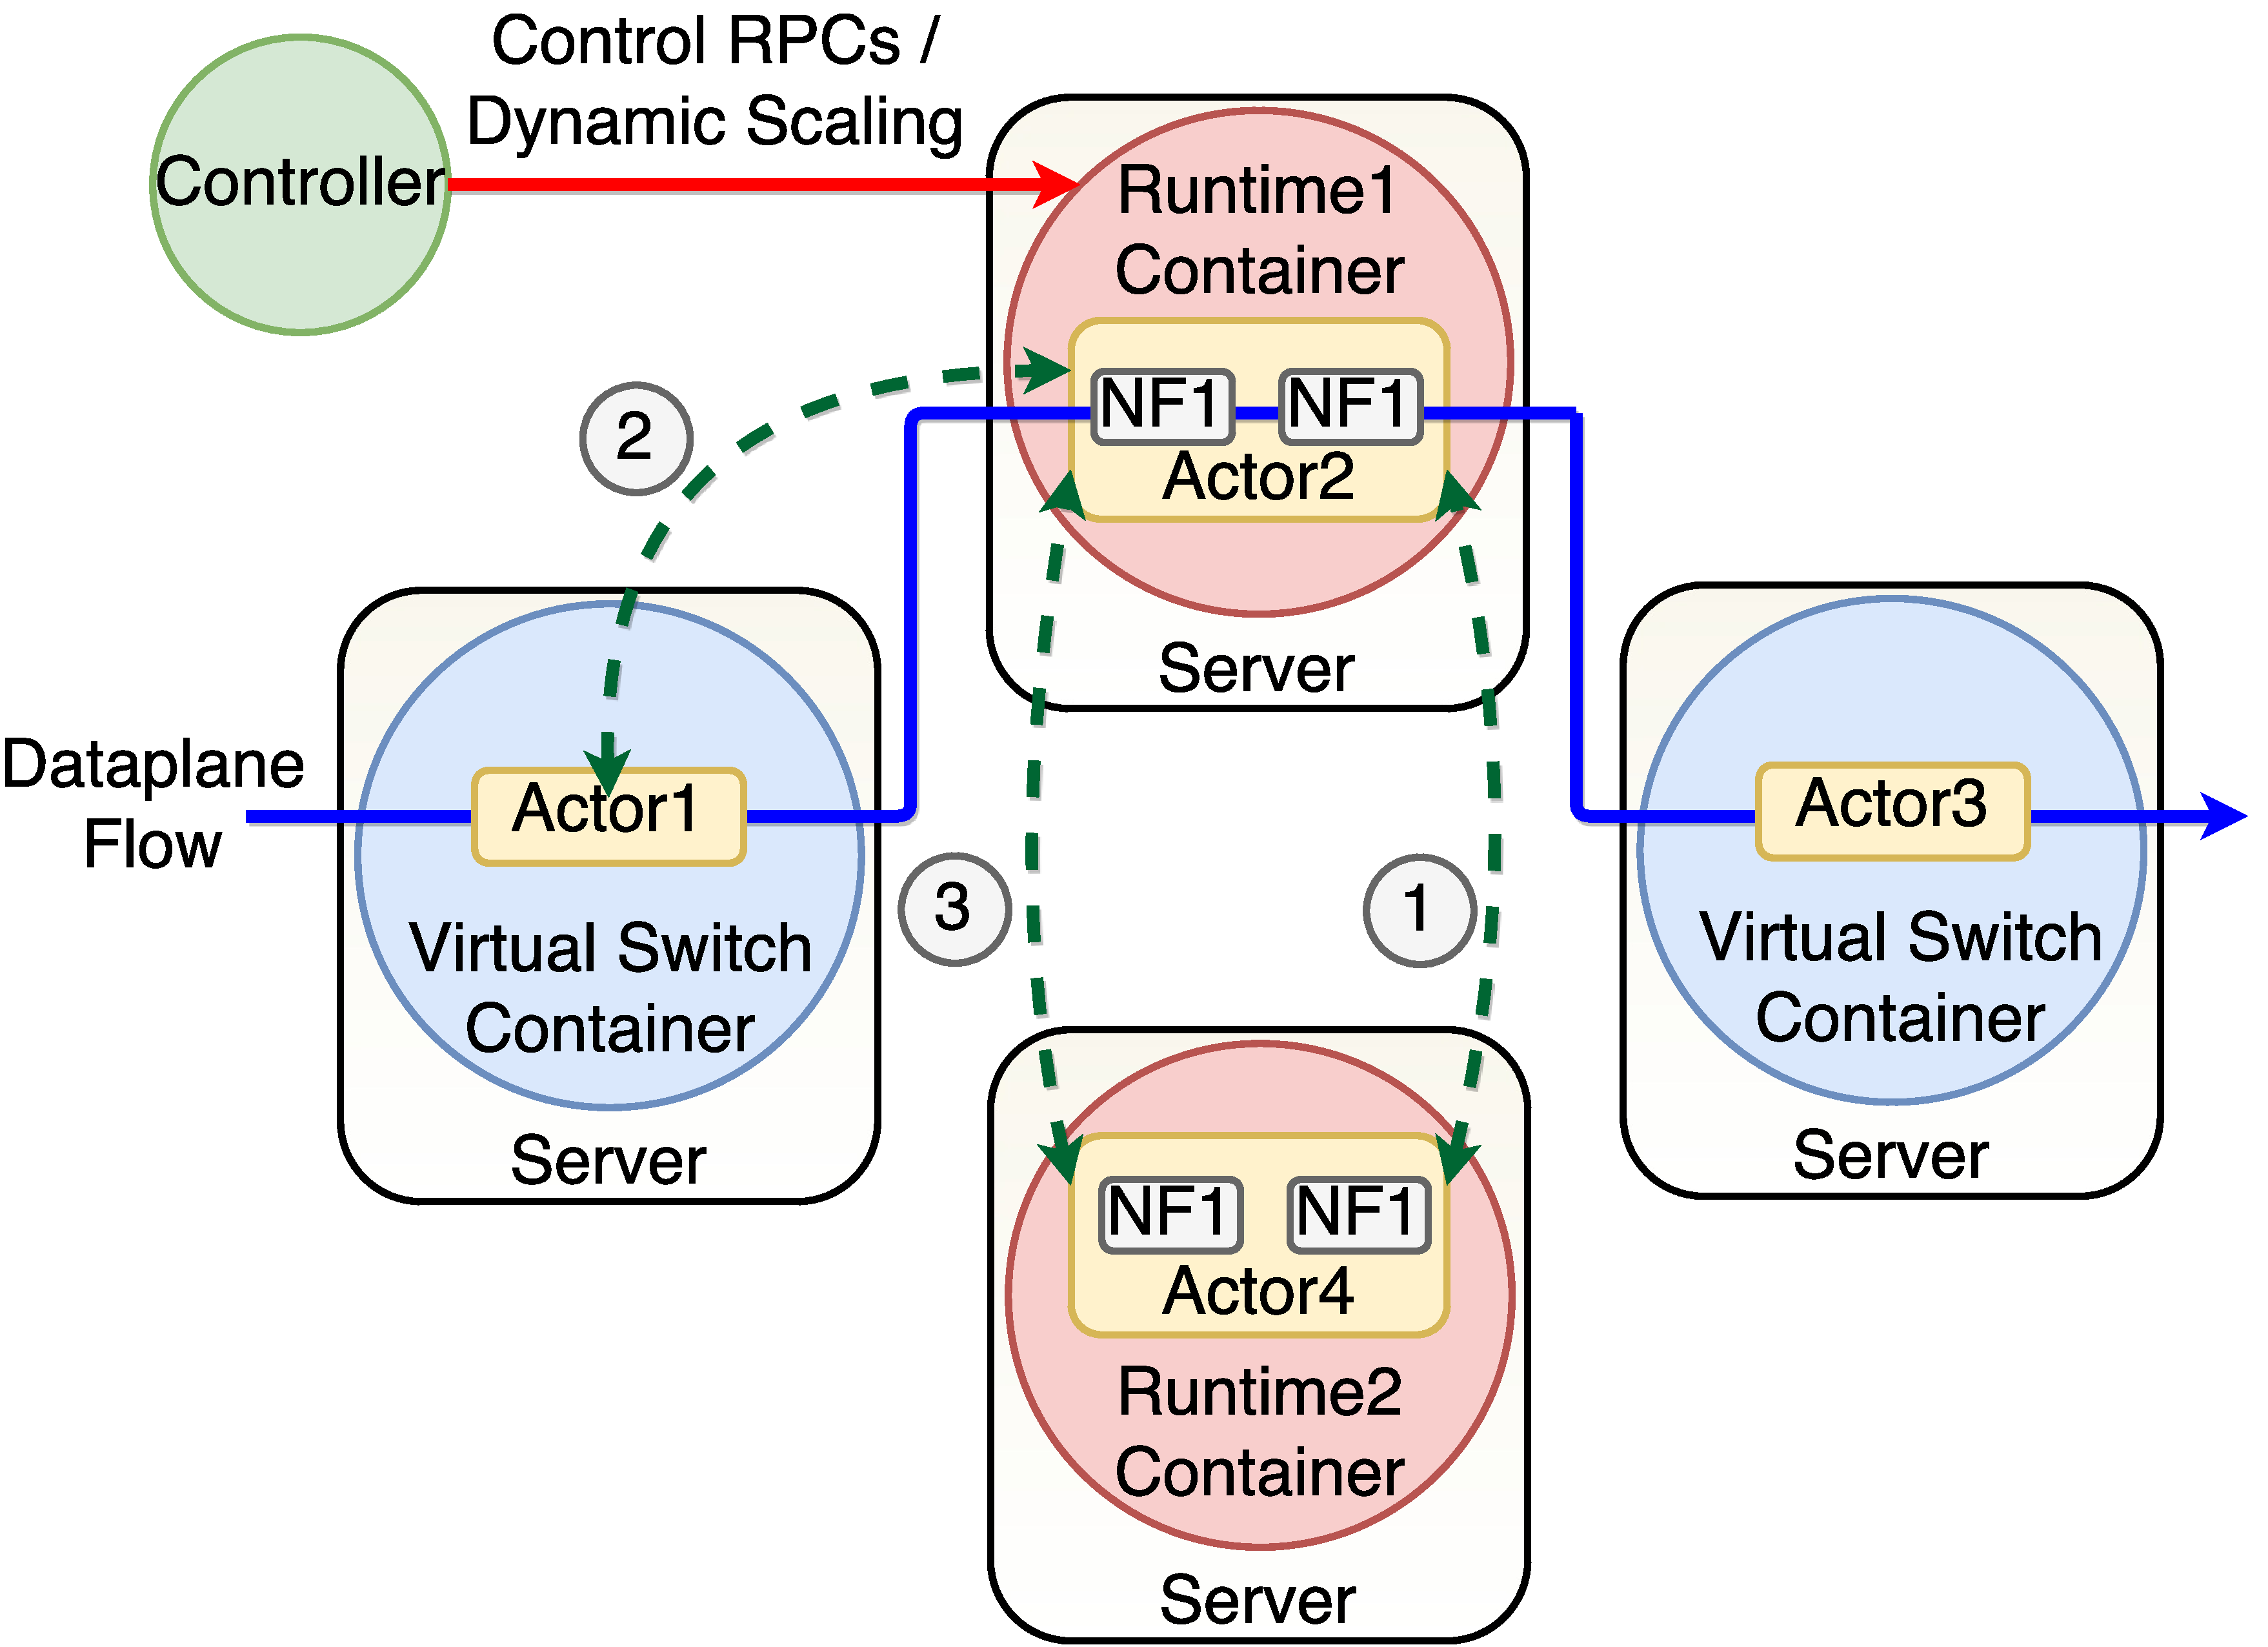
\includegraphics[width=\columnwidth]{figure/final-final-nfactor-cluster.pdf}
  \caption{An overview of NFActor framework.}
  \label{fig:runtime}
\end{figure}

Figure \ref{fig:runtime} demonstrates the basic architecture of NFActor framework, consisting of a light-weight controller, input and output virtual switches and several runtime systems (referred to as \textit{runtime} in short). NFActor framework runs virtual switches and runtimes inside containers, so that they can be quickly rebooted in case of failure and elastically scaled in case of overload.

The incoming dataplane flows are first sent to the input virtual switch, which dispatches them to runtimes. Each runtime hosts a NF service chain that is determined during runtime initialization phase and conducts the actual serivce chain processing. When a runtime receives a new flow, it creates a new actor and delegates the packet processing of the flow to that actor. The actor loads all the required NF modules of the service chain when it is created and passes the received flow packet to these NF modules in sequence. Once the service chain processing is finished, the actor sends the packet to an output virtual switch, where the packet is sent to its final destination.

One of most significant features that differentiate NFActor framework with existing works \cite{gember2015opennf} is that flow management tasks is fully automated without the need of a centralized controller. In figure \ref{fig:runtime}, actor 2 in runtime 1 could migrate itself to actor 4 on runtime 2, by exchanging 3 messages with actor 1 and actor 4. The decentralized nature of NFActor framework originates the micro execution context built for each flow.

A controller does exists in NFActor framework, which is a relatively light-weighted one. It's tasks are to monitor the workload of each runtime and control dynamic scaling. It's only appearance when executing flow management tasks is during the initiation phase, where it uses control RPCs to tell the flows which runtime they should migrate to.

\section{NF Module API}

\begin{figure}[!h]
\begin{subfigure}[t]{0.49\linewidth}
   \centering
   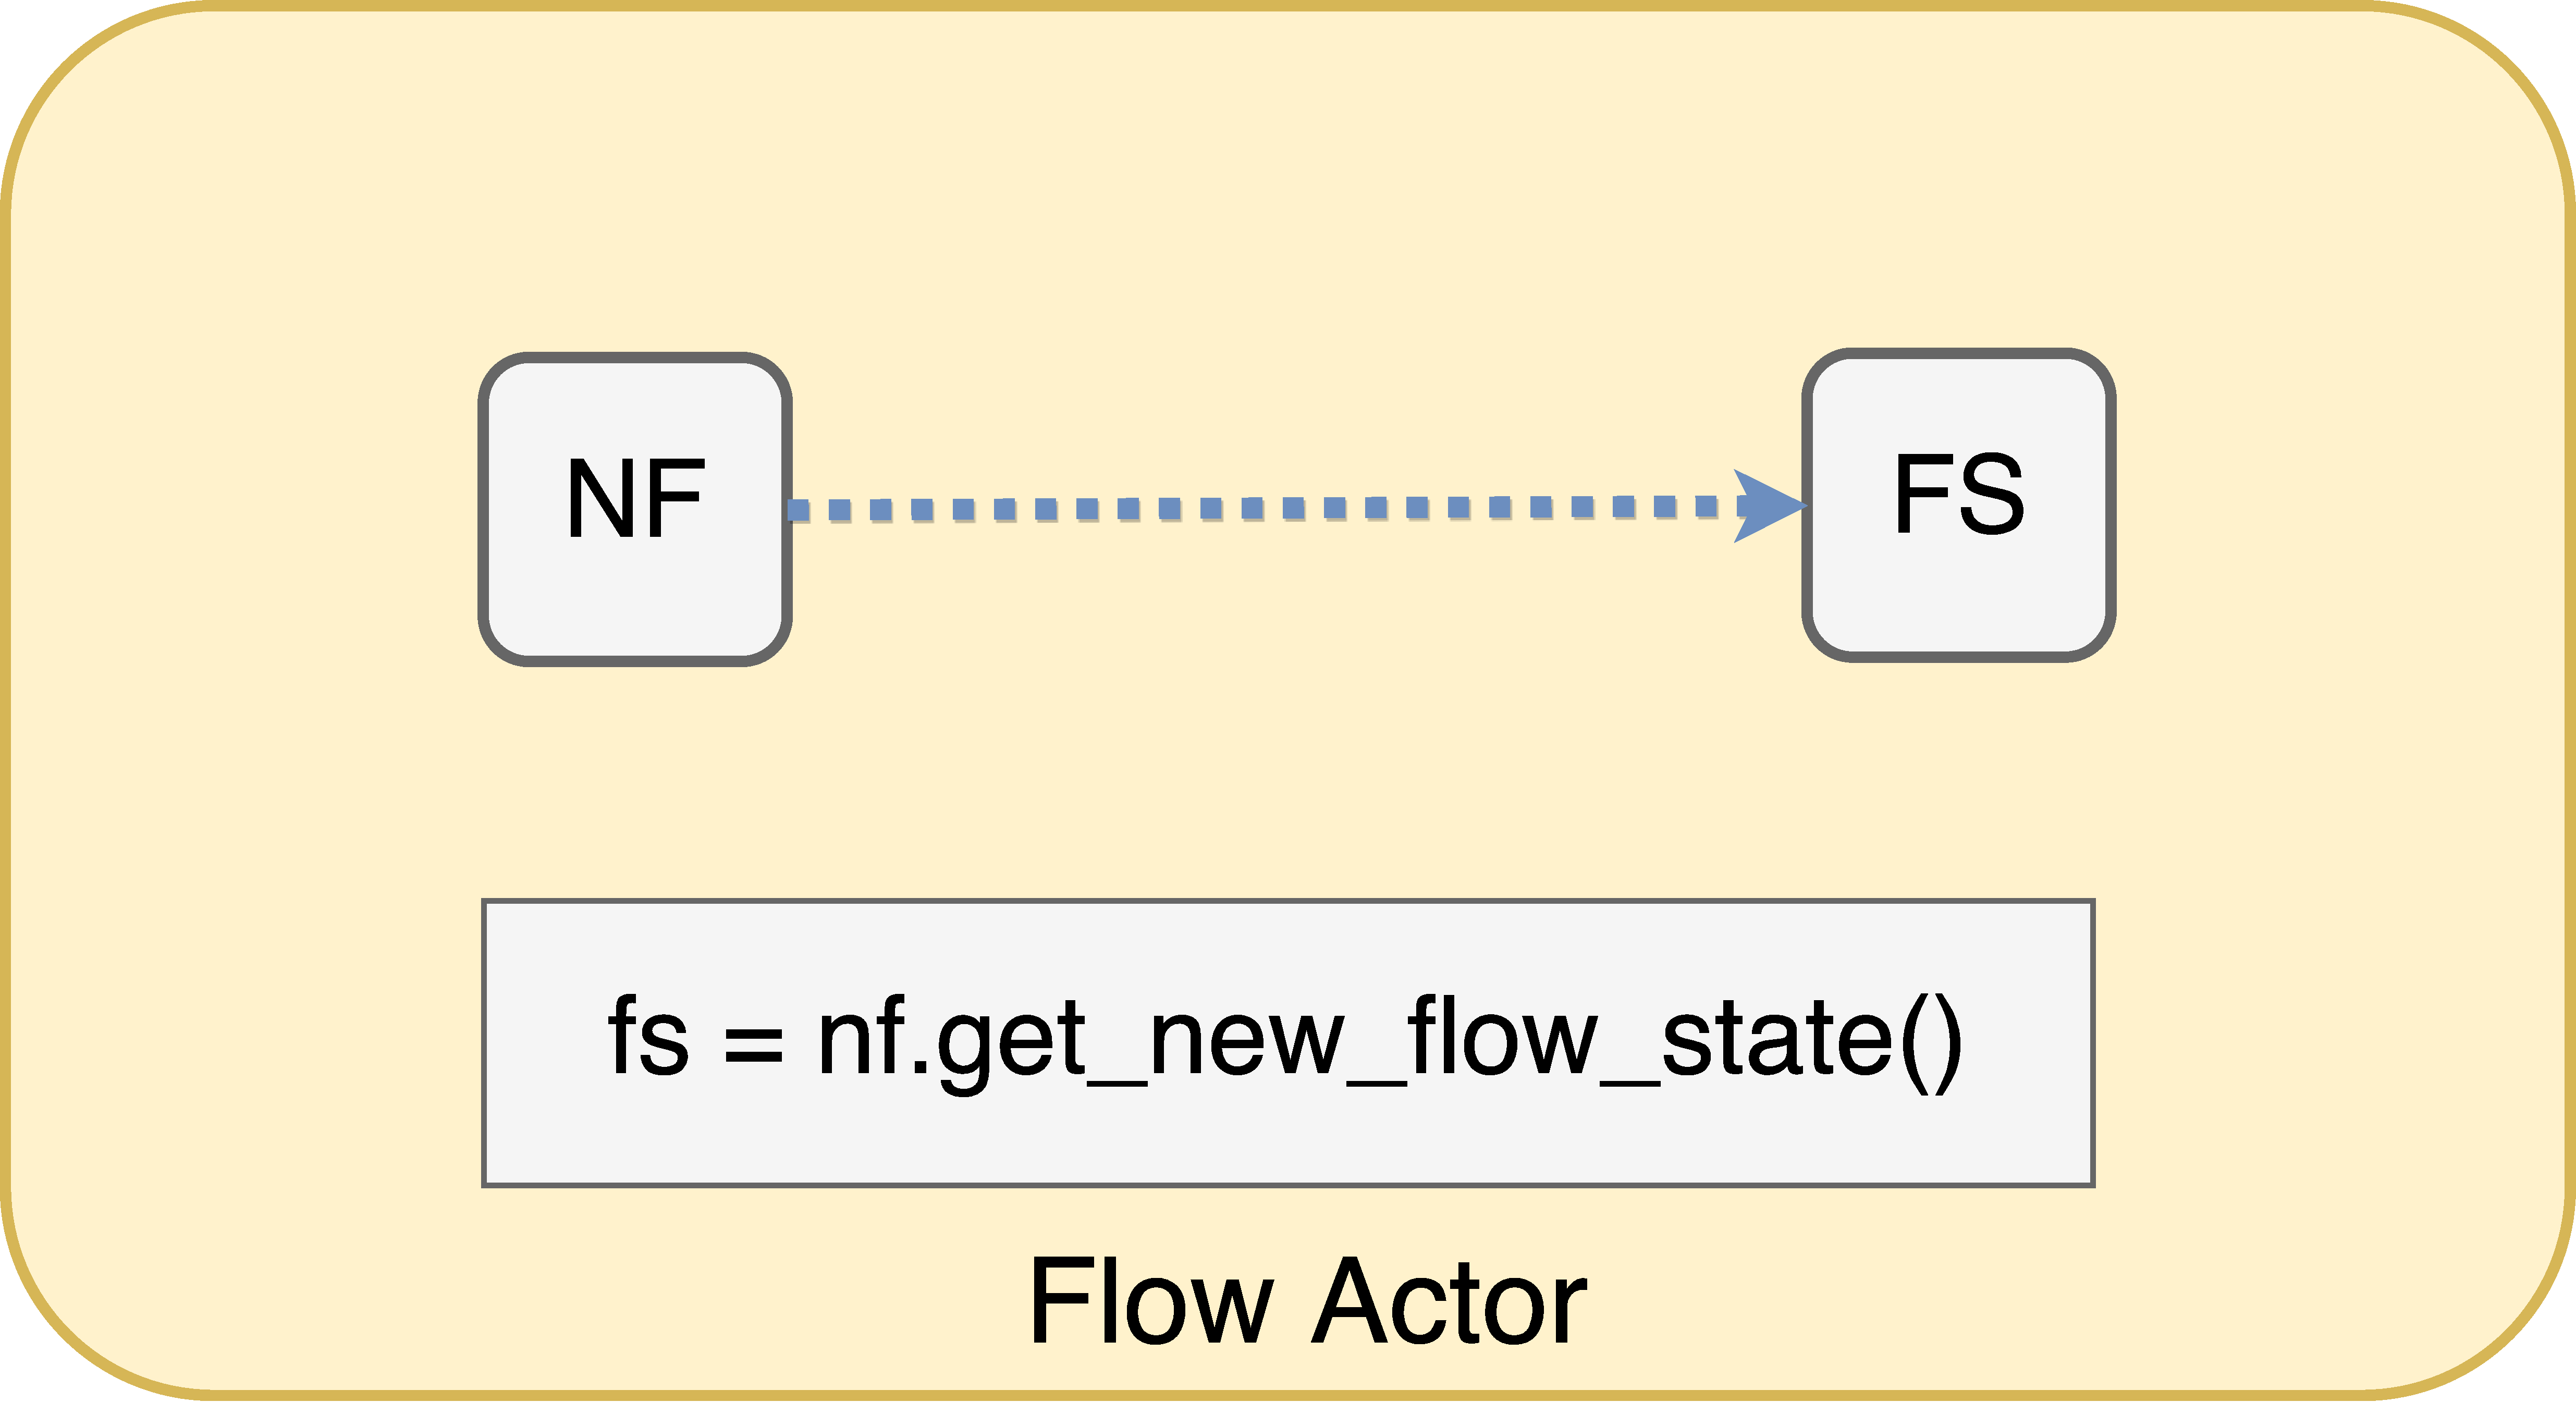
\includegraphics[width=\columnwidth]{figure/nf-module-api-init.pdf}
   \caption{The API that is used to initialize flow state when the flow actor is created.}\label{fig:init-api}
  \end{subfigure}\hfill
  \begin{subfigure}[t]{0.49\linewidth}
 \centering
   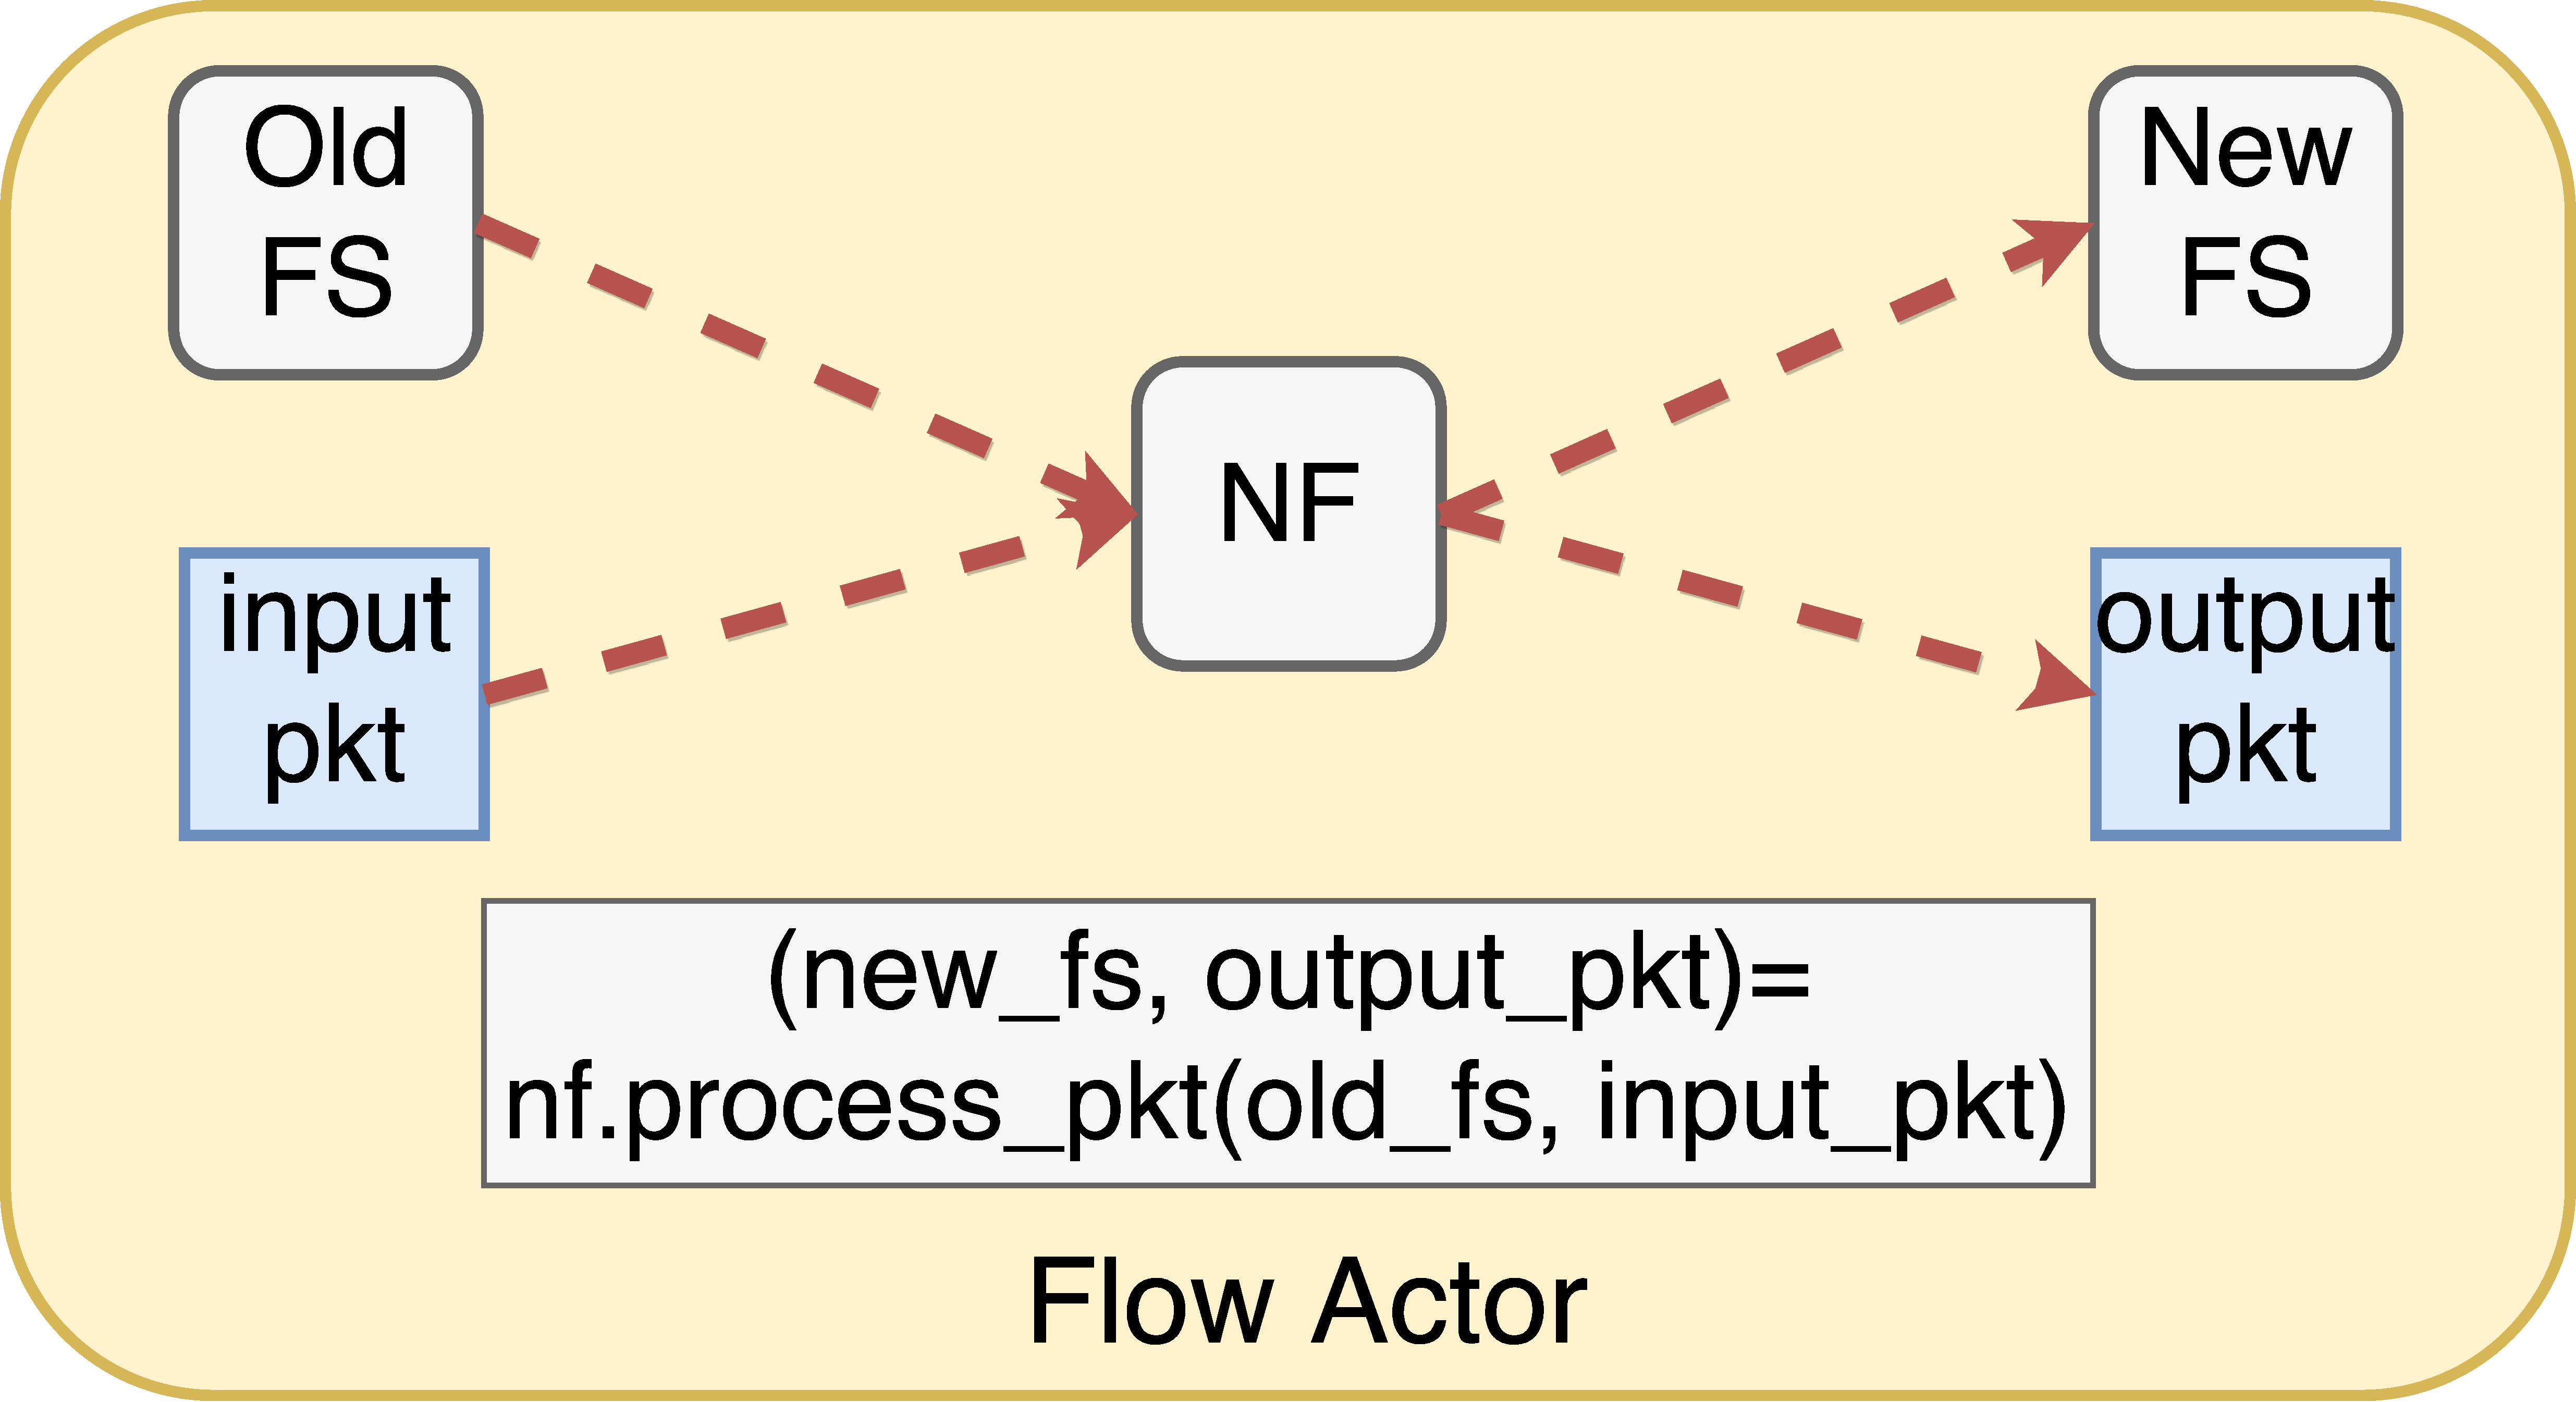
\includegraphics[width=\columnwidth]{figure/nf-module-api-process_pkt.pdf}
   \caption{The API that is used to process input packet.}\label{fig:pkt-process-api} \end{subfigure}\hfill
 \caption{The API exposed by NFActor for implementing new NF modules. (NF: Network function. FS: Flow state. pkt: packet.)}
\label{fig:api}
\end{figure}

Each NF used by NFActor is implemented as a loadable module. The runtime system could select which NF module to load and use. In order to achieve the service chain processing as indicated in figure \ref{fig:runtime-arch}, we pass in an argument indicating the composition of the service chain before initializing a runtime. The runtime guarantees that each flow actor processes the packet through each NF as indicated in the service chain. The modular NF design is similar to that in NetBricks \cite{199352}, however, NFActor modifies the interface exposed by the NF module to achieve efficient flow management.

When executing flow management tasks, flow actor must be able to extract and transmit the flow states of all the NFs on the service chain, without disturbing the normal service chain processing. To speed up this process, we propose to separate the flow state with the processing logic of the NF module, and store the flow state inside the flow actor.

We summarize the core APIs used by NFActor to construct new NF modules in figure \ref{fig:api}. Using these APIs, the flow actor could acquire a new flow state when it is created. When the flow actor processes a packet, the flow actor passes the current flow state and the input packet together into the processing logic of a NF module. The processing logic could directly update the flow state according to the input packet. Since the flow state is stored by the flow actor, the flow actor could directly manipulate its flow state when executing flow management tasks, without disturbing the NF processing logic.

Even though this design facilitates flow management tasks, it has its own limitation. Using this design, it is hard to extract and tranismit shared states. However, it is a complicated tasks to guaratee the consistency of shared states when managing a single flow. It may require multiple synchronizations, thereby affecting the processing speed of a single flow management task. Sice our primary goal when designing NFActor is to provide a high performance exeuction context, we do not aim to synchronize shared state. Instead, when flow management affects the consistency of the shared state, we could explicitly notify the NF about the result of flow management tasks and let NF module to handle the inconsistecy.

%\section{Runtime Architecture}

\subsection{Runtime}
\label{sec:runtime}

\begin{figure}
		\centering
		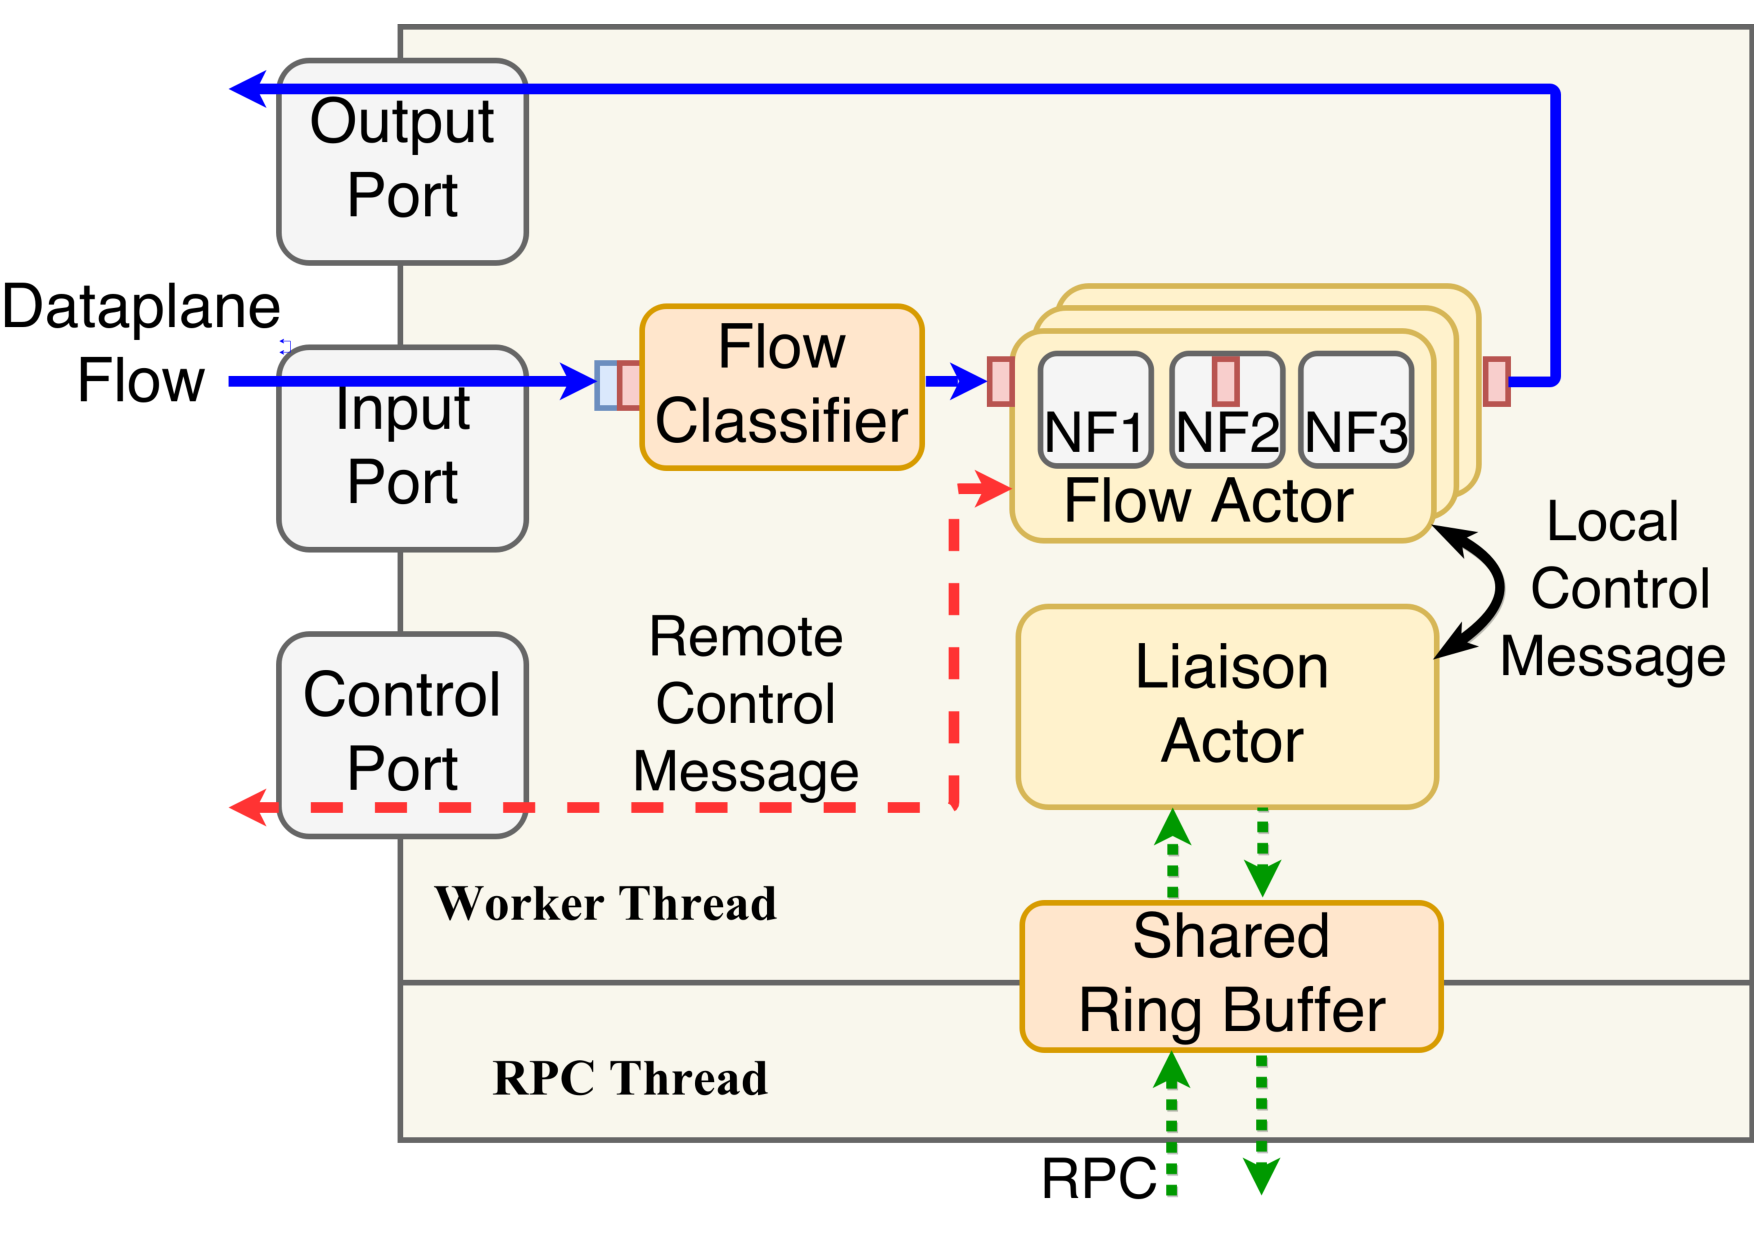
\includegraphics[width=\columnwidth]{figure/new-nfactor-runtime-arch.pdf}

		\caption{The internal structure of a runtime in \nfactor.}
\label{fig:runtime-arch}
\end{figure}

The concept of a uniform runtime system, as a basic flow processing and scaling unit in \nfactor, does not appear in most existing work \cite{bremler2015openbox, gember2012stratos, palkar2015e2}. In existing NFV systems, the basic flow processing and scaling unit is an NF instance, which is a virtual machine or container hosting an instance of a NF. % and the NF instances are chained on the data-plane. % The flows must go through these NF instances in sequence. 
 The primary reason that we design such a runtime is to enable NFs/service chains to achieve failure resilience automatically without coordinator intervention, as the runtime provides a network transparent abstraction \chuan{change this `network transparent' to a more accurate wording} to communicate and exchange messages among each other, which are crucial for flow migration and replication. 
  Especially, in a runtime, we adopt the simple yet powerful design to create a micro execution context for each flow, and encapsulate processing functions of the flow over its entire service chain inside the micro execution context. Then we can enable failure resilience on the basis of each micro execution context (Sec.~\ref{sec:resilience}). To be able to process multiple flows, the runtime is capable of handling multiple micro execution contexts concurrently. 

In \nfactor, we exploit the actor programming model to implement the micro execution context. Each micro execution context is a flow actor. Flow processing by NFs in the service chain, flow migration and replication functionalities are all implemented as message handlers of the flow actor. The runtime provides the basic runtime environment for all the flow actors that it has created. 


Fig.~\ref{fig:runtime-arch} shows the internal structure of a runtime. The input and output ports are used for receiving and sending flow packets from and to virtual switches. The control port is used for transmitting and receiving control messages exchanged among different runtimes for flow migration and replication, which are directly encapsulated inside L3 packets and sent/received using DPDK. %Both input port and output port could be used transmit and send actor messages as well, for instance, during the second request-response in the flow migration and during flow recovery.
 Input packets of dataplane flows are first sent to a flow classifier, which uses the classical 5-tuple of a flow (\ie, source IP address, destination IP address, transport-layer protocol, source port and destination port) to identify packets belonging to the same flow. One flow actor is created for each new flow. The flow actor loads NFs of the service chain configured in the runtime. All packets of the same flow are sent to the same flow actor, which processes them in sequence by passing them through NFs in the service chain. 
 
Each runtime is configured with a specific service chain by the coordinator during its booting phase. The runtime installs and initializes all the NFs as specified in the service chain upon booting. When a flow actor is created, it loads these NFs and uses a number of carefully defined NF APIs, as given in Table \ref{table:api} in Sec.~\ref{sec:NFAPIs}, to allocate flow states \chuan{not clear what `allocate flow states' means. extract?} and xxx \chuan{describe what it does to facilitate flow migration and replication by rewriting the idea of the following sentence: `Besides service chain processing, the flow actor also provides an execution context for distributed flow migration and replication, in response to certain messages (Sec.~\ref{sec:resilience})'}. 


Each runtime can host one or multiple flow actors for flows passing through the same service chain that the runtime is configured with, depending on its resource availability and performance isolation requirements. In case of a multi-tenant NFV system, we can run actors processing flows of the same tenant on the same runtime, but those of different tenants on different runtimes, for better security and isolation. When multiple flow actors are concurrently running on one runtime, they are scheduled by a worker thread: \chuan{clearly describe how the flow actors are scheduled} whenever a message is received at the actor's mailbox, .... In addition, our design of the NF modules in the next section will show that passing packets to a NF for processing in a flow actor is essentially just a function call; only one copy of each NF software needs to be loaded in a runtime, while the flow actors can all make use of it. %An actor itself is a very lightweight one as millions of actors could be spawned in seconds \cite{chs-rapc-16}. 



The runtime also consists of a RPC thread for receiving RPC requests from the coordinator (for flow migration, replication, etc.) and responding to them. The RPC thread and the worker thread share a ring buffer, used for relaying RPC requests received by the RPC thread to a liaison actor in the worker thread. We use a high-speed shared ring buffer to achieve fast inter-thread communication \chuan{add citation}. The liaison actor is responsible for coordinating with flow actors to execute the RPC requests from the coordinator. % flow actor initialization, flow migration and flow replication. %Flow actor and coordinator actor could directly exchanges local messages, or exchange remote messages through a reliable message passing module \cite{}.





\vspace{1mm}
\noindent {\bf Discussions on Runtime Design Choices.} The design of supporting only one service chain in one runtime significantly reduces the overhead of installing many NFs and avoids service chain selection in one runtime, for higher packet processing efficiency (speed) and management simplicity. Our one-actor-one-flow design is useful for facilitating fast flow migration (Sec.~\ref{sec:resilience}), which migrates a flow by migrating the actor that processes it \chuan{revise to more accurate description}. There are a few possible alternatives to our one-actor-one-flow design: (1) {\em One flow actor handles multiple flows.} It compromises the efficiency of flow migration, especially when multiple flows come from different virtual switch actors. In this case, the flow actor must synchronize the responses sent from different virtual switch actors \chuan{clarify what are `responses sent from different virtual switch actors' and why the flow actor needs to sync them}, adding overhead to flow migration process. (2) {\em One flow actor runs one NF}. Additional overhead is needed for chaining multiple flow actors to constitute a service chain, lowering packet processing speed. %Therefore, the one-flow-one-actor design achieves a sweet point in minimizing the actor processing overhead and improving the efficiency of flow migration protocol design.
Instead of using multiple worker threads in a runtime, the single-worker-thread design guarantees a sequential execution order of flow actors, thereby completely eliminating the need to protect message passing by locks \chuan{message passing among flow actors or what?}, and achieving higher efficiency. 




%The alternative design to one-runtime-one-service-chain is to dynamically configure multiple service chains on a single runtime. Then due to the one-flow-one-actor design, we need to do an additional service chain selection, based on some pre-defined rules. This adds additional overhead to the flow actor processing and increases the complexity when managing the NFActor cluster, because the controller must populates the service chain rule dynamically to each runtime. With the one-runtime-on-service-chain design, if another service chain is needed, the system administrator could launch a new NFActor cluster and configure a different service chain to use.




%The runtime is designed as a single-worker-thread architecture to decrease the overhead of flow actors. A high speed NFV system may process millions of packets every second and migrates tens of thousands of flows. At such a high processing rate, message passing protected by shared lock in multi-threaded actor runtime system may incur a huge overhead and hurt the packet throughput.
%The runtime is configured with a specific service chain during the boot phase and initializes all the NF modules as specified in the service chain. When a flow actor is created, it loads these modules and uses the flow state allocation method \ref{table:api} to allocates all the
%To process flows across a service chain, during the initialization phase of the runtime, a service chain specifier is passed in to the runtime. The runtime then loads all the NF modules as indicated in the service chain specifier. When the flow classifier creates a new flow actor, the flow actor also loads these NF modules on the service chain and passes the input packet along the NF modules in sequence.

%The reason that the runtime is designed as a single-worker-thread program is because the multi-worker-thread design may not bring significant performance gain. In our initial prototype implementation, we use LIBCAF \cite{caf} library to construct flow actors. LIBCAF library creates multiple worker threads and schedules flow actors to run on these worker threads. Because LIBCAF completely conceals the internal interfaces of the worker threads, we have to create a dedicated polling thread to poll packet from the input port. Under this design, we find that the maximum throughput of a runtime does not increase when the number of LIBCAF worker thread increases, because the polling thread has always been a bottleneck. Therefore, we abandon the multi-worker-thread design and use a single worker thread to poll packets and schedule flow actors. To our surprise, this architecture turns out to work very well because it allows us to perform aggressive optimization of actor programming model \ref{}. In the mean time, we can still maintain the scalability of the system by launching more runtimes.

\subsection{NF APIs}
\label{sec:NFAPIs}

To achieve transparent resilience together with the micro execution environments provided by runtimes in \nfactor, an important step is to separate useful NF states from the core processing logic of each NF. With this separation, a flow actor can retrieve and serialize NF states for transmission whenever needed, without interfering with packet processing of the NF. In \nfactor, we achieve this separation by designing a set of APIs that NF implementation should follow in \nfactor. 
 
\begin{table}[!t]
\centering
\caption{APIs to be Implemented by NFs in \nfactor.}
\label{table:api}
\resizebox{\columnwidth}{!}{
\begin{tabular}{c|l}
\textbf{API}                                      & \multicolumn{1}{c}{\textbf{Usage}}                                                                                                                                                                                                         \\ \hline
nf.allocate\_new\_fs()                            & \begin{tabular}[c]{@{}l@{}}Create a new flow state object for\\ a new flow actor, to be used for storing flow state\end{tabular}                                                                                                                                                  \\ \hline
nf.deallocate\_fs(fs)                             & \begin{tabular}[c]{@{}l@{}}Deallocate the flow state object\\ when the flow actor expires\\\end{tabular}                                                                                                                               \\ \hline
nf.process\_pkt(input\_pkt, fs)                   & \begin{tabular}[c]{@{}l@{}}Process the input packet using the \\ current flow state\end{tabular}                                                                                                         \\ \hline
%nf.get\_migration\_target(cluster\_cfg, fs) & \begin{tabular}[c]{@{}l@{}}Query an NF using the current\\ cluster configuration and \\ flow state about which runtime this flow\\ actor should be migrated to\end{tabular} \\ \hline
\end{tabular}
}
\end{table}


The APIs are given in Table \ref{table:api}, provided as four public methods for each NF to implement. When a new flow actor is created to handle a new flow, it first calls $nf.allocate\_new\_fs()$ to create a flow state object. Whenever the actor receives a new packet, the actor passes the received packet and the flow state object to \\
$nf.process\_pkt(input\_pkt, fs)$, for processing by the NFs, in sequence of the service chain. Any changes to the flow state when an NF has processed the packet is immediately visible to the flow actor. When the flow terminates, the flow actor expires and it calls $nf.deallocate\_fs(fs)$ to deallocate the flow state object. Using these three APIs, the flow actor always has direct access to the latest flow state, enabling it to transmit the flow state during flow migration and replication processes without disturbing packet processing of the NFs. %Therefore, the combination of the three methods servers as the basis for the transparent resilience in~\nfactor. 

%\chuan{add the idea to flow migration section rather than exposign the API here} The fourth API $nf.get\_migration\_target(cluster\_cfg, fs)$ is used for checking where the NF would like the actor to migrate to, by passing the current cluster configuration and the current flow state. This enables the flow actor to actively migrate itself instead of waiting for migration initiation command sends from the controller \ref{}. This distributed design is the key to sparkle several useful applications, \ie, flow deduplication and reliable MPTCP subflow processing, which we will discuss in Sec.~\ref{sec:experiments}, that existing NFV systems based on centralized flow management cannot achieve. The flow actor should only call this method on the last NF in the service chain. Therefore NFs modules implementing this method should be placed on as the last NF in the service chain. 

%These three methods are simple to use and properly generalize the structure of NFs that processes flow packets based on per-flow state. Using these three methods, we are able to create several representing NFs as shown in \ref{}.}

%The flow actor acquires the flow state of all the NF modules using the allocation API, and passes the packet across all the NF modules in sequence using the processing API.


To implement an NF in \nfactor, core processing logic of the NF needs to be implemented following the actor model and the APIs in Table \ref{table:api}. Nevertheless, porting the core
processing logic of an existing NF software is relatively straightforward. We have implemented a broad range of NFs in \nfactor and will present details in Sec.~\ref{sec:experiments}.


\subsection{Virtual Switch}
\label{sec:virtualswitch}

A virtual switch in \nfactor~is a special runtime where the actors do not run a service chain but only a load balancer function. Following the one-actor-one-flow principle, a virtual switch can create multiple actors each to dispatch packets belonging to one flow. We refer to a flow dispatching actor in a virtual switch as a {\em virtual switch actor}. 


Each virtual switch receives information of the runtimes that it can dispatch flows to from the coordinator, through RPC requests its liaison actor receives, including MAC addresses of the input ports of the runtimes. A virtual switch actor selects one of the runtimes to forward its flow in a round-robin fashion, upon creation of this actor. We choose a simple round-robin approach because the virtual switch must run very fast and a round-robin algorithm introduces the smallest amount of overhead while providing satisfactory load balancing performance. Whenever a virtual switch actor receives an incoming packet, it replaces the destination MAC address of the packet to MAC address of input port of the chosen runtime, modifies the source MAC address of the packet to MAC address of output port of the virtual switch, and then sends the packet out from the output port.

The architectural consistency of virtual switches and runtimes in \nfactor~facilitates flow migration and replication. The flow actor on a runtime can analyze the source MAC address of the incoming packets and determine which virtual switch this packet comes from. Then the flow actor can contact the virtual switch during flow migration and replication processes, to indicate change of the runtime that the respective virtual switch actor should dispatch packets to. This is done through remote control message exchanges with the virtual switch in the same way as message exchanges with other runtimes.

\chuan{describe how the virtual switches are used for receiving outgoing packets from runtime and send them to final destinations}

Existing NFV management systems either rely on SDN switches \cite{gember2012stratos, gember2015opennf} to route flows from one NF to the next, or build a customized data-plane for inter-connecting different NF instances \cite{palkar2015e2}. In comparison, our virtual switch is lightweight, only to dispatch flows to runtimes, but not route flows through individual NFs.


\subsection{Coordinator}
\label{sec:coordinator}

The \nfactor's coordinator is responsible for launching new virtual switches and runtimes, monitoring the load on each runtime and executing dynamic scaling. Due to our distributed flow actor design, the coordinator only needs to participate in the initiation phase of flow migration and replication (Sec.~\ref{sec:resilience}). This differentiates \nfactor's coordinator with the controllers in existing NFV systems \cite{gember2015opennf}\cite{rajagopalan2013split}, which need to fully coordinate the entire flow migration process. 
The design of the coordinator is simplified and improve failure resilience of the system is improved, as the coordinator does not need to maintain complicated states associated with flow migration.

To deploy a service chain in \nfactor, the system administrator first specifies composition of the service chain to the coordinator, as well as several rules to match the input flows to service chains. \chuan{describe how you use SDN or openflow like rules to enable dispatching flows to correct virtual switches}. The coordinator then launches a new virtual switch and a new runtime, configures the runtime with this service chain, and directs incoming flows using the service chain to the virtual switch. Each runtime or virtual switch is assigned a global unique ID to ease management.  In \nfactor, a virtual switch is responsible for dispatching flows using the same service chain, to runtimes installed with this service chain. The virtual switches and runtimes handling the same service chain are referred to as a {\em cluster} in \nfactor. Flow migration and replication occur within a cluster. These design choices are made since xxx \chuan{give the rationale}.


Each runtime in \nfactor~regularly sends heartbeat messages to the coordinator, containing the current load information (\ie, CPU usage, memory usage) of the runtime. When the coordinator detects that a runtime is overloaded, it scales up the cluster by launching a new runtime and configures the service chain on that runtime (Sec.~\ref{}\chuan{point to the scaling section}). \chuan{does the coordinator takes care of virtual switch scaling as well? describe it}

The coordinator communicates with runtimes via a series of control RPCs exposed by each runtime, as summarized in Table \ref{table:rpc}. It uses $PollWorkload()$ to acquire the current load on a runtime, to produce scaling decision. The coordinator maintains the composition of the system, which includes the mac addresses of input/output/control ports and the IDs of all runtimes and virtual switches of all clusters (handling different service chains). The coordinator updates a runtime composition of the runtime it belongs to using $NotifyClusterCfg(cfg)$ \chuan{does coordinator sends it to virtual switches as well?}. The cluster composition learned by different runtimes in a cluster do not have to be consistent because our flow migration and replication protocols perform safety checking by exchanging requests and responses to eliminate the inconsistency \chuan{check if this is true and revise accordingly}. The last three RPCs are used to initiate flow migration and replication. After issuing these three calls, migration and replication are automatically executed without further involving the coordinator.
\chuan{briefly describe why you use RPC for coordinator to runtime communication.}



\begin{table}[!t]
\centering
\caption{Control RPCs Exposed at Each Runtime}
\label{table:rpc}
\resizebox{\columnwidth}{!}{
\begin{tabular}{l|l}
Control RPC                                                                                   & Functionality                                                                                                                                              \\ \hline
PollWorkload()                                                                                   & \begin{tabular}[c]{@{}l@{}}Poll the load information \\ from a runtime.\end{tabular}                                                                 \\ \hline
NotifyClusterCfg(cfg)                                                                         & \begin{tabular}[c]{@{}l@{}}Notify a runtime the current \\ cluster view.\end{tabular}                                                             \\ \hline
\begin{tabular}[c]{@{}l@{}}SetMigrationTarget(runtime\_id, \\ migration\_number)\end{tabular} & \begin{tabular}[c]{@{}l@{}}Initiate flow migration. It tells \\ the runtime to migrate \\ migration\_num of flows to the runtime\\ with runtime\_id.\end{tabular} \\ \hline
SetReplica(runtime\_id)                                                                       & \begin{tabular}[c]{@{}l@{}}Set the runtime with runtime\_id \\ as the replica.\end{tabular}                                                                \\ \hline
Recover(runtime\_id)                                                                          & \begin{tabular}[c]{@{}l@{}}Recover all the flows replicated \\ from runtime with runtime\_id.\end{tabular}                                                 \\ \hline
\end{tabular}
}
\end{table}
\section{Implementation}
\label{sec:implementation}


%\nfactor~is implemented in C++ using a combination of DPDK \cite{dpdk}, BESS module system \cite{bess} and GRPC \cite{grpc}.
The core functionalities of \nfactor~ are implemented by about $8500$ lines of code in C++, except the code for NFs. We customize an actor library, and run our runtimes and virtual switches on Docker containers \cite{docker}. We use BESS \cite{bess} as the dataplane inter-connection tool for connecting different runtimes and virtual switches, building a virtual L2 network inside each server, and connecting each virtual L2 network to the physical L2 network connecting all the servers. The three ports in each runtime are BESS ZeroCopy VPorts - high-speed virtual ports implemented with DPDK for fetching and transmitting raw packets. With DPDK, the memory holding packet buffers is mapped directly into the address space of the runtime process, %xxx\chuan{complete},
avoiding high context switching overhead if using the traditional kernel network stack and speeding up packet handling \cite{martins2014clickos}. %By connecting the virtual L2 ethernet with the ports of runtimes,~\nfactor connects runtimes running on different server together.

\vspace{1mm}
\noindent \textbf{Resource Allocation to Runtimes.} %To use BESS VPort, the container that hosts a runtime must be configured with the highest system access right (set $--previledge=true$). Therefore each container actually could uses all the CPU cores on the server.
When launching runtimes on one server, the coordinator ensures that the worker threads of the runtimes are pinned to different CPU cores (excluding core 0 and the cores that are used by BESS), since they are busy polling threads which keep the CPU utilization to 100\%. The RPC threads of all the runtimes in the same server are collective pinned to core 0, since they sleep for most of the time waiting for RPC requests.  %The threshold for identifying whether a runtime overloads is set to 100 dropped packet on the input port of the runtime over one second.

%\subsection{Customized Actor Library}
%\label{sec:actor-library}
\vspace{1mm}
\noindent \textbf{Customized Actor Library.} We implement our own actor library, including a fast actor memory allocator, a fast actor timer and a set of C++ base classes for implementing new actors. %xxx \chuan{summarize what this library includes}.
In this actor library, due to our single-worker-thread design, local actor message transmission is directly implemented as a function call, therefore eliminating the overhead of enqueuing and dequeuing messages to and from an actor's mailbox \cite{actor-wiki}. For remote actor message passing, we assign a unique ID to each actor. A sender actor only needs to specify the receiver actor's ID and the hosting runtime's ID, and then the reliable transmission module (to be discussed soon) can correctly deliver the remote actor message to the receiver actor. We also implement a flow actor scheduler, % in the first three tasks of the worker thread. The flow actor scheduler
 which redirects both input flow packets and remote actor messages to corresponding flow actors, by looking up the flow actors using the 5-tuple.
 Even though functionalities provided by our customized actor library are much simpler than those in the existing actor frameworks \cite{akka} \cite{caf}, its simple design leads to effective actor processing overhead reduction, enabling high-speed packet processing. %Our customized actor library could not achieve complicated ac as other mature actor frameworks do \cite{akka} \cite{caf}. However, due to its simple architecture, it only imposes a small overhead when doing actor processing, therefore it is able to satisfy the high-speed packet processing requirement of modern NFV system.




%We decide to reuse BESS module systems. BESS module system is specifically designed to schedule packet processing pipelines in high-speed NFV systems, which is a perfect suit to~\nfactor runtime architecture. We port the BESS module system and BESS module scheduler to the runtime and implement all the actor processing tasks as BESS modules. All the implemented BESS modules are  scheduled inside worker thread to achieve flow actor scheduling, packet processing over the service chain and remote actor message transmission.

%\chuan{moved to runtime section} The worker thread routinely carries out the following four tasks. (i) Poll dataplane packets from intput/output port, run a actor schedule to schedule flow actors to process these packets and sends the packets out from the output/input port after flow actors finishes processing the packets. (ii) Poll packets from control ports, reconstruct packet stream into remote actor messages and send the actor messages to the receiver actors. (The first task also carries out similar processing as the second task because remote messages are also sent to input/output port as shown in Sec.~\ref{sec:resilience}). (iii) Run the liason actor to process RPC requests sent from the coordinator and dispatches flow migration initiation messages to active flow actors in the runtime. (iv) Fetch remote actor messages from a queue that are enqueued by actors during the execution of previous three tasks and send the remote actor messages out from the three ports.

%\begin{itemize}

%\item The first/second pipeline polls packets from the input/output port, runs actor scheduler on these packets and sends the packets out from the output/input port.

%\item The third pipeline polls packets from control ports, reconstruct packet stream into remote actor messages and send the actor messages to the receiver actors. (The first/second pipeline also carries out this processing because remote messages are also sent to input/output port \ref{}).

%\item The fourth pipeline schedules coordinator actor to execute RPC requests sent from the controller. In particular, coordinator actor updates the configuration information of other runtimes in the cluster and dispatches flow migration initiation messages to active flow actors in the runtime.

%\item When processing the previous four pipelines, the actors may send remote actor messages. These messages are placed into ring buffers \ref{}. The fifth pipeline fetches remote actor messages from these ring buffers and sends remote actor messages out from corresponding ports.

%\end{itemize}

%The runtime uses BESS scheduler to schedule these 5 pipelines in a round-rubin manner to simulate a time-sharing scheduling.



%\subsection{Reliable Message Passing Module}
%\label{sec:ReliableMsgPassing}
\vspace{1mm}
\noindent \textbf{Reliable Remote Actor Message Passing.}
Actor messages passed among flow actors on different runtimes should be reliably delivered. We build a customized reliable message passing module, which inserts those messages into a reliable byte stream for transmission. % to the other end, the reliable message passing encodes messages into reliable packet streams.
The module creates one ring buffer for each remote runtime and virtual switch. When a flow actor on this runtime sends a remote actor message, the module creates a packet, copies the content of the message into the packet and then enqueues the packet into the respective ring buffer. %A message may be split into several packets. %and different messages do not share packets.
These packets are configured with a sequential number each, and appended with a special header to differentiate them from dataplane packets.
The worker thread dequeues these packets from the ring buffers, and sends them to respective remote runtimes. A remote runtime acknowledges receipt of such packets. Retransmission is fired in case that the acknowledgement for a packet is not received after a configurable timeout (\eg, 10 times the RTT).

Since our goal is to reliably transmit remote actor messages over an inter-connected L2 network, we do not use user-level TCP \cite{jeong2014mtcp}, %\chuan{reference missing in .bib, your project code url is also missing in .bib},
which may impose much more processing overhead for reconstructing byte streams into messages.
In addition, packet-based reliable message passing provides additional benefits during flow migration and replication. Because the response in 2nd request-response step of flow migration is sent as a packet using the same path as the dataplane packets, reliable actor message passing enables us to implement loss-avoidance migration with ease (Sec.~\ref{sec:migration}).
%I will remove this claim, I forgot that we still need to do packet copy.
%During flow replication, we can directly send the output packet as a message to the replica actor, without the need of additional packet copy \chuan{I do not get what additional packet copy might be needed}.

%\subsection {Worker Thread}
%\label{sec:BessModuleSys}
\vspace{1mm}
\noindent \textbf{Worker and RPC Threads.}
The worker thread on a runtime polls packets from the ports, schedules flow actors and transmits remote actor messages (Sec.~\ref{sec:runtime}). To schedule these tasks efficiently, we implement them as BESS modules and use the BESS module scheduler, which schedules these modules in a round-robin fashion. Each worker thread is pinned to one CPU core to avoid overhead due to OS scheduling. % and improve packet processing performance.
 The RPC thread on each runtime is implemented with GRPC \cite{grpc}, and the RPC requests are sent over a reliable TCP connection between a runtime and the coordinator.

%I'm about to move it to evaluation secition.
%\subsection{New Applications}

%We also build several applications based on \nfactor, which exploits its lightweight, distributed flow migration capability to achieve useful functionalities. %, including live NF update, reduce output bandwidth for deduplication NF and ensure reliable and safe MPTCP processing. We evaluate and demonstrate these new applications in our evaluation.

%\noindent\textbf{Live NF update.} %NF often needs to be updated (\eg, software version, important NF configuration files), existing systems would typically migrate flows away, stop the NF and then relaunching it.
% \nfactor~can achieve dynamic NF update (\eg, software version, important NF configuration files) without interfering active flows running on a runtime by dynamically migrating the flows out to a replica runtime, performing update and migrating the flows back. We show in the evaluation that the dynamic update ensures no active flows are dropped during the update.


%\noindent\textbf{MPTCP sub-flow processing.} When a MPTCP \cite{} flow traverses an NFV system, its sub-flows may be sent to different NF instances for processing. Some network functions require all subflows to be processed by the same instance, \eg, xxx \chuan{is this the problem of subflows being processed by different instances?}. %because they have different flow-5-tuple and appear as different flows on the virtual switch.
%In \nfactor, we can add a MPTCP sub-flow detection function to each flow actor, such that when the flow actor processes the first packet of a flow, it can check whether it belongs to a MPTCP flow. If so, the flow actor performs a consistent hashing using the MPTCP header to decide a migration target runtime in the cluster, and migrates the flow to the target. In this way, different sub-flows belonging to the same MPTCP flow can be processed by the same flow actor. This is hard to be achieved in existing NFV systems without signicant central coordination. %, since flows can not initiate active migration request by themselves.

%The final application is similar with MPTCP application, which reduces the output bandwidth for deduplication.
%\noindent\textbf{Efficient Flow Deduplication.} Flow deduplication, as an important functionality of WAN optimizers \chuan{add citation}, is useful for reducing bandwidth consumption due to transfer redundant data across different flows. \nfactor~can efficiently support flow deduplication: when a runtime receives a flow, it checks for duplicated content contained in the flow packet \chuan{how does it check duplicated content among different flows received on different runtimes?}. In case it finds out the duplication, the flow actor initiates a migration to move the flow to a specific runtime \chuan{how to decide this specific runtime}. In this way, duplicated flows can be processed on the same runtime, eliminating the output bandwidth on each runtime \chuan{why processing duplicated flows on the same runtime can reduce output bandwidth? Are they processed by the same flow actor? what if the flows are partially duplicated but not entirely?}. This is hard to be achieved in existing NFV systems because xxx \chuan{give the reason}.

\section{Experiments}
\label{sec:experiments}


We evaluate \nfactor~using a cluster of around 10 Dell R430 servers, each containing 20 logical cores, 48GB memory and 2 Intel X710 10Gb NICs. The servers are connected through a 10GB switch. We implement a number of NFs using the APIs in Table \ref{table:api}: firewall (336 LOC), IDS (734 LOC), load balancer (47 LOC), flow monitor (169 LOC), HTTP parser (1471 LOC) and a NF for MPTCP subflow detection (223 LOC, which is used for experiments in Sec.~\ref{sec:applications}). %Among these 5 NFs, the first three carry out light-weight tasks where as the later two carry out heavy-weight tasks.
The firewall maintains several rules such as blocking a certain source IP address,
and checks each received packet against the rules: if the packet violates any of the rules, a tag in the flow state is flipped and later packets are automatically dropped. The firewall also records the TCP connection status of the flow in the flow state. The IDS is a simplified version of Snort IDS \cite{snort}.
The flow monitor updates an internal counter whenever it receives a packet. The HTTP parser parses received packets for HTTP requests and responses, and saves them together with the HTTP method in the flow state object. %Throughout the evaluation, we use a service chain consisting of  ``flow monitor$\rightarrow$firewall$\rightarrow$http parser'' as the service chain. We generate evaluation traffic using the BESS's FlowGen module and we directly connect the FlowGen module to the external input port of the virtual switch.

We run at most $50000$ actors per runtime according to memory allocation of the runtimes. % performs a pre-allocation of the memory to store actors for processing speed and does not grow the allocated memory.
The coordinator updates cluster composition to runtimes and virtual switches once every 5 seconds.
Each collective buffer at a migration target runtime can store up to 4096 DPDK packets.% 32768 bytes, capble of storing 4096 DPDK packet pointers.
A runtime is identified as overloaded if more than $100$ packet drops are recorded on the input port of the runtime within one second.
%The algorithm uses 500 flows are used as the number of flows for migration number, which is a tunable value in~\nfactor. We use this value because 500 flows could be migrated within one millisecond in~\nfactor and the coordinator could gradually increases the workload during migration to evenly balance the workload.

%The rest of the section tries to answer the following questions. \textit{First, } what is packet processing throughput of~\nfactor, does it scales well? \textit{Second,} how good is the flow migration performance of~\nfactor when compared with existing works like OpenNF? \textit{Third,} how is the performance of flow replication? \textit{Fourth,} how good is~\nfactor's dynamic scaling algorithm performs. The section concludes with the performance of the unique applications that are enabled through~\nfactor's distributed flow migration.

%how well can~\nfactor~scales, in terms of the number of runtimes running inside the system? (Sec.~\ref{sec:normal})

%what is the packet processing capacity of \nfactor~framework? (Sec. \ref{sec:ppc}) \textit{Second, } how well is \nfactor~scales, both in terms of the number of worker threads used by a runtime and the number of runtimes running inside the system? (Sec. \ref{sec:ppc}) \textit{Third, } how good is the flow migration performance of \nfactor~framework when compared with existing works like OpenNF? (Sec. \ref{sec:fmp}) \textit{Fourth, } what is the performance overhead of flow state replication and does the replication scale well? (Sec. \ref{sec:rp})

\subsection{Packet Processing Throughput}
\label{sec:ppc}


%\begin{figure}[!t]
%	\centering
%	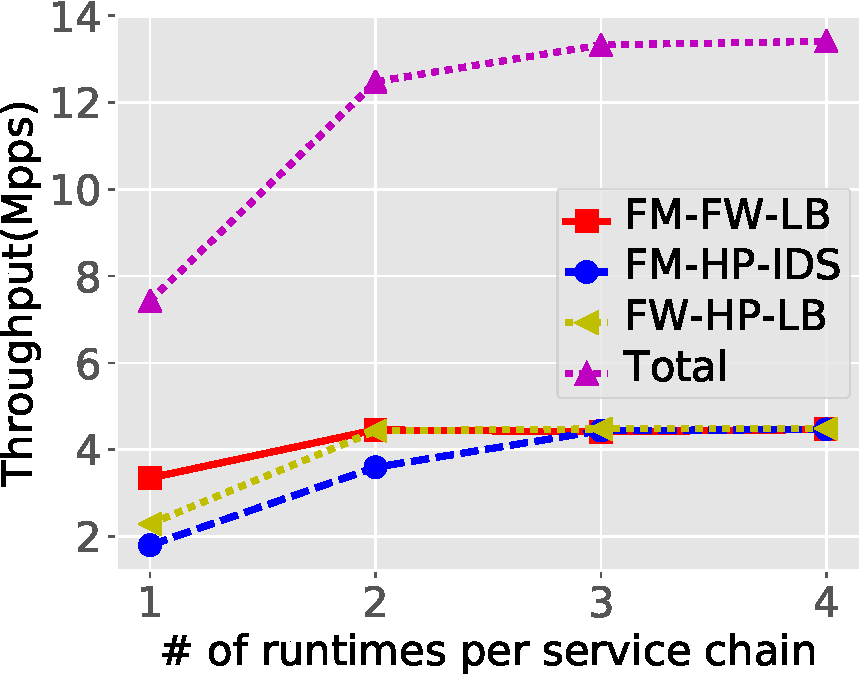
\includegraphics[width=\columnwidth]{figure/revised-throughput-test.pdf}
%	\caption{Packet processing throughput.}
  %(\textbf{FM}: Flow Monitor. \textbf{HP}: HTTP Parser. \textbf{FW}: Firewall. \textbf{LB}: Load Balancer. \textbf{IDS}: Intrusion Detection System.)
%\label{fig:normal-case-eval}
%\end{figure}

\begin{figure}[!t]
 \begin{subfigure}[t]{0.475\linewidth}
   \centering
   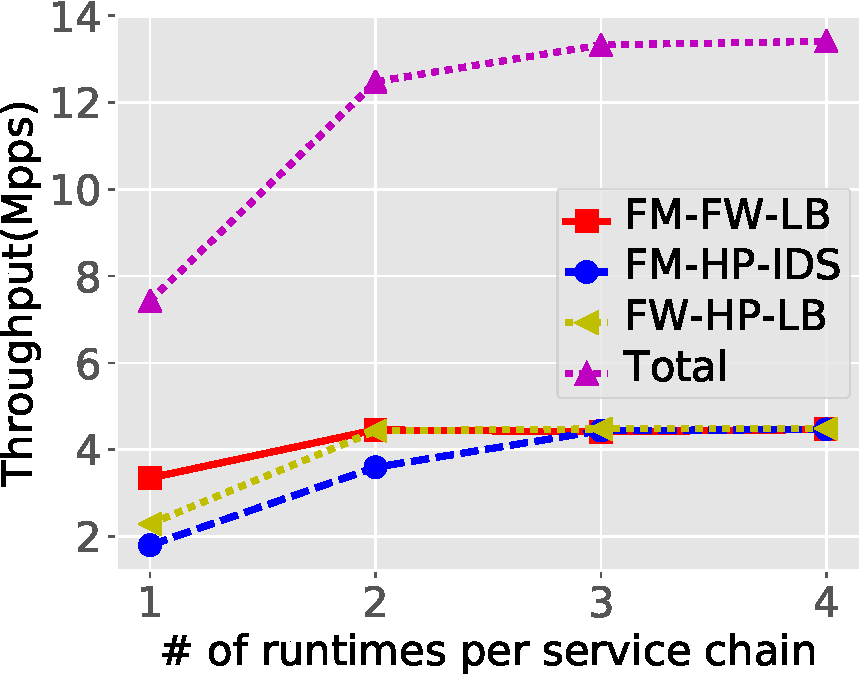
\includegraphics[width=\columnwidth]{figure/revised-throughput-test.pdf}
   \caption{}\label{fig:normal-case-eval} \end{subfigure}\hfill
  \begin{subfigure}[t]{0.505\linewidth}
   \centering
   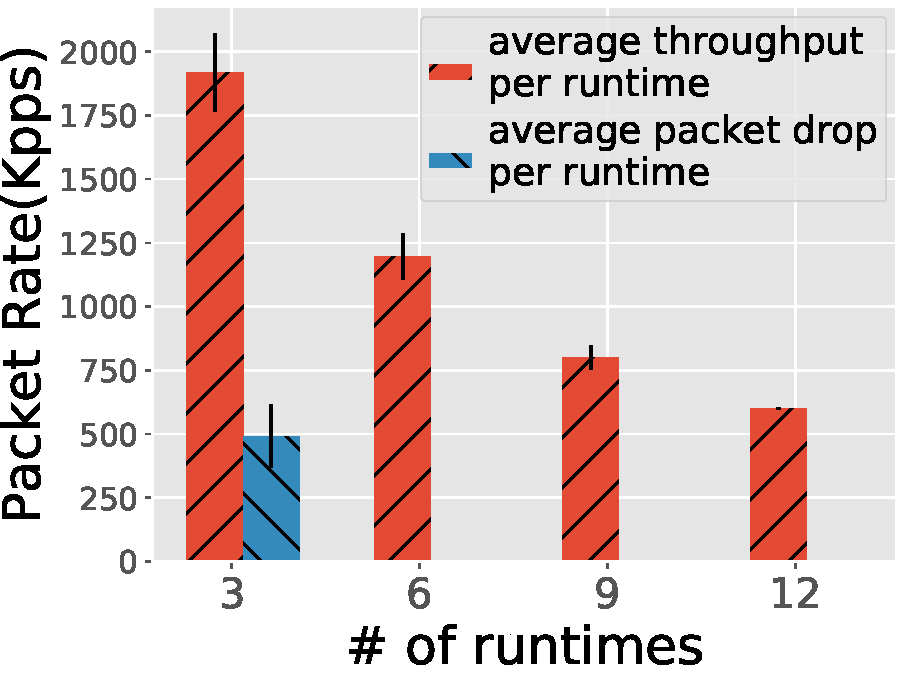
\includegraphics[width=\columnwidth]{figure/Mixtest.pdf}
   \caption{}\label{fig:mix-work-flow}
  \end{subfigure}
\caption{ Packet processing throughput.} %(a) The total time to migrate different numbers of flows concurrently on three runtimes. (b) The flow migration performance of NFActor. Each flow in NFActor runtime goes through the same service chain as in Figure \ref{fig:tot-mig}. OpenNF controlls PRADS asset monitors. The flow packet rate is 20pps.}
\label{fig:mig-perf}
\end{figure}



 %\begin{figure}[!t]
%	\begin{subfigure}[t]{0.49\linewidth}
%		\centering
%		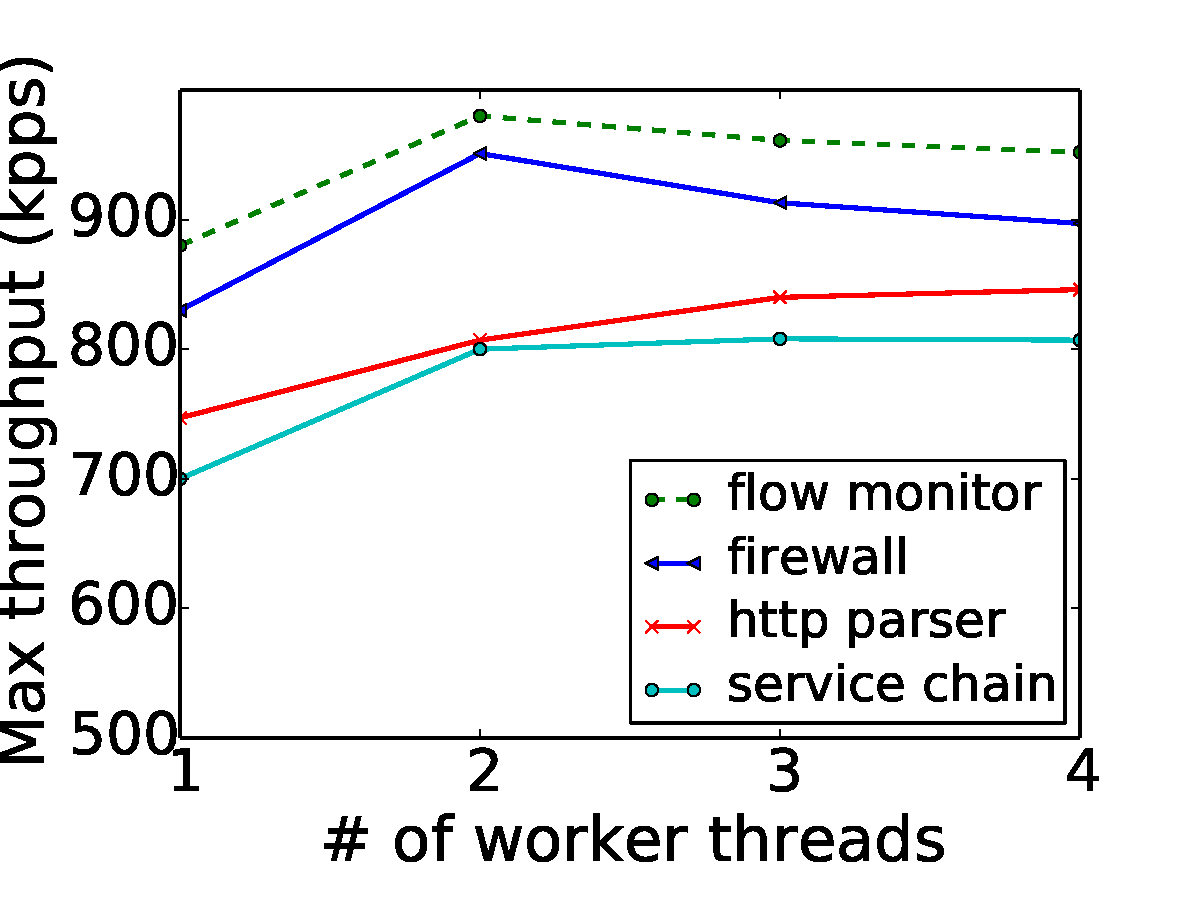
\includegraphics[width=\columnwidth]{figure/nf_throughput_evaluation.pdf}
%		\caption{Packet processing capacity of a single \nfactor~runtime system running with different number of worker threads.}\label{fig:normal-performance} \end{subfigure}\hfill
%	 \begin{subfigure}[t]{0.49\linewidth}
%		\centering
%		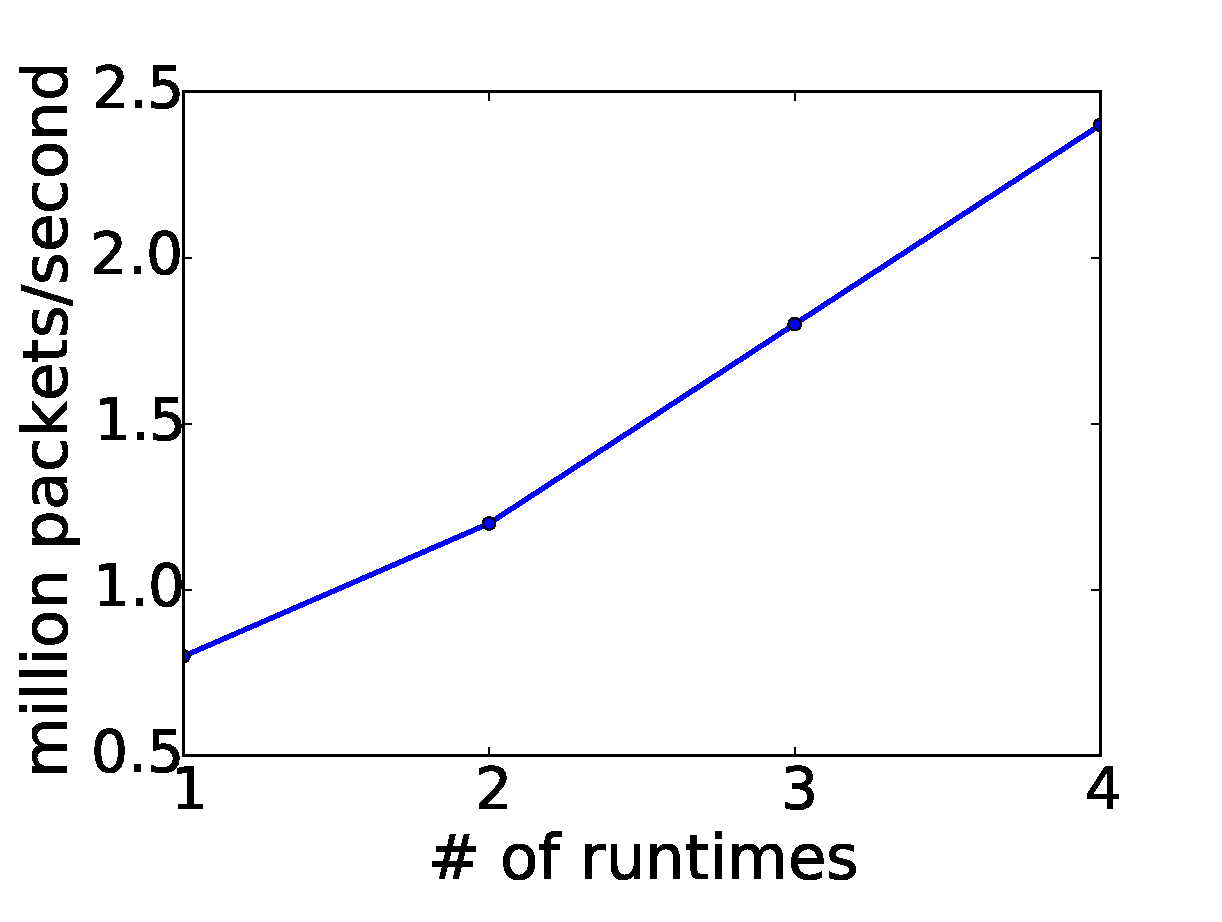
\includegraphics[width=\columnwidth]{figure/runtime_pktthroughput.pdf}
%		\caption{Aggregate packet processing capacity of several \nfactor~runtimes.}\label{fig:scalability-performance}
%	 \end{subfigure}
%\caption{The performance and scalability of \nfactor~runtime, without enabling flow migration }
%\label{fig:performance}
%\end{figure}

We run six virtual switches on one server for dispatching flows to runtimes, run runtimes on other servers, and implement a traffic generator to produce flows to be sent to virtual switches. The flows consist of 64 byte data packets. We deploy three service chains, `flow monitor (FM) $\rightarrow$ firewall (FW) $\rightarrow$ load balancer (LB)', `flow monitor (FM) $\rightarrow$ HTTP parser (HP) $\rightarrow$ IDS', and `flow monitor (FM) $\rightarrow$ HTTP parser (HP) $\rightarrow$ load balancer (LB)'.\footnote{\nfactor~can handle service chains with branches similarly, due to encapsulating each service chain entirely in one flow actor and the run-to-completion scheduling strategy in runtimes. We evaluate simle service chains without branches which represent the mainstream \cite{hwang2015netvm, martins2014clickos}.} The same number of flows are processed by each of the service chains. We do not enable flow replication in this set of experiments. % and use the same number of runtimes to process packets for each service chain.


We first evaluate the packet processing throughput of \nfactor~using uniform flows, each produced at 10pps (packets per second), lasting for 10 seconds. We inject an overall rate of all flows around $14Mpps$ (60K flows) into virtual switches, %\chuan{14*64*8=7168, why is this close to line rate of 20Gbps for the two NICs of a server? Answer: because on the ethernet, the size of the packet is increased to larger than 80bytes.}
 which approaches line-rate of the server NICs. We evaluate the throughput when different numbers of runtimes are deployed for each service chain. %Since each runtime can handle at most 50000 flows, we scale up the number of runtimes with the increase of flows.

%For each service chain, we run two traffic generators to generate traffic into the service chain, resulting in a maximum throughput at around 4.4Mpps.


Fig.~\ref{fig:normal-case-eval} shows that %all flows using each service chain can be timely processed.
 when there are more than 2 to 3 runtimes for each service chain, the total packet processing capacity of the runtimes is larger than the incoming flow rate (about $14Mpps$), leading to a stablizing overall throughput about $14Mpps$.  %starting with 2 or 3 runtimes implies that the amount of the input traffic injected into the service chains is smaller than the total packet processing capacity of these service chains when each of these two chains are scaled with more than 2 runtimes. %The total throughput of \nfactor when handling three service chains easily scale up to around 14Mpps, which basically saturate a 10Gb NIC card, therefore achieving line-rate throughput. Therefore~\nfactor can scale well and satisfies the line-rate processing requirement of modern NFV system.
 In addition, we start to observe zero packet loss for all the three service chains when the number of runtimes is scaled up to 3.



 We next evaluate packet processing throughput with flows whose duration spans 10 seconds to one minute, %, with a 10 second step. The
 %flow arrival rate varies from 1000 flows to 5000 flows \chuan{why do you need to vary the flow arrival rates? I think this experiment should be done using static total flow numbers; you can comment this clause out andrevise the total number of flows injected to the concurrent number},
flow rate varies from 1kpps to 2kpps, %with a 1000-flow step.
 and packet size varies among 64 bytes, 128 bytes and 256 bytes. The total number of injected flows is 550K.
 The runtimes are configured with a service chain `flow monitor $\rightarrow$ HTTP parser $\rightarrow$ IDS'. Fig.~\ref{fig:mix-work-flow} shows the average throughput and packet drop of each runtime, when different numbers of runtimes are deployed for each service chain. An error bar indicates the standard deviation. We can see that the flow processing load is quite balanced among different runtimes (using our simple round-robin scheduling algorithm) and the runtimes can handle all the incoming flows when the number of runtimes is scaled up to six (zero loss). The primary reason that the round-robin algorithm used by the virtual switch balances workload well enough even in case of non-uniform flows is because the total number of injected flows are large enough (550K), which is a common case for high-speed NFV system. 

These results exhibit high efficiency of the runtime design and flow migration protocol in \nfactor. % enabling close to line-rate flow processing. % good packet processing performance achieved by~\nfactor is primarily due to our efficient actor design.
 The development of \nfactor~has gone through a few trials and errors. In our previous version of \nfactor~design and prototype implementation using Libcaf \cite{caf}, we used 4 worker threads per runtime. Compared with the old design, our current design with one worker thread per runtime can achieve up to 4x throughput. We believe the reason is that the customized actor library and the single worker thread design completely eliminate the overhead of multi-threaded contention for shared resource, \ie actor's mailbox. % enabling current version to out-perform the previous version.

% We believe the reason is that the combination of our customized actor library and the DPDK-based reliable message passing eliminates a lot of overhead associated with actor processing. \chuan{the reason you gave is not relevant to 4 worker threads per runtime}
%The traffic generator generates  generate the same amount of traffic to each service chain.  using differnt number of runtimes, running three service chains. The traffic generators generates flows each lasts for 10 second with a 20 pps (packet per second) flow rate. The packet size is 64 byte. We increase the number of concurrently generated flows to generate packets at around 14Mpps, reaching NIC line-rate. We set up different number of runtimes and configure runtimes with different service chains and calculate the cumulative packet rate from all the runtimes. From \ref{fig:normal-case-eval}, we can see that the runtime in~\nfactor can scale almost linearly and achieve almost line-rate processing when scaled up to 9 runtimes. Therefore,~\nfactor has good packet processing throughput and can satisfy the stringent requirement of modern NFV system.

% reach   with a uniform We can see that the packet processing throughput scales almost linearly as the number of runtime increases, until normal case performance of running \nfactor~framework. Each flow in the generated traffic has a 10 pps (packet per second) per-flow packet rate. We vary the number of concurrently generated flows to produce varying input traffics. In this evaluation, we gradually increase the input packet rate to the \nfactor~cluster and find out the maximum packet rate that the \nfactor~cluster can support without dropping packets. In figure \ref{fig:normal-performance}, the performance of different NF modules and the service chain composed of the 3 NF modules are shown. Only one \nfactor~runtime is launched in the cluster. It is configured with different number of worker threads. In figure \ref{fig:scalability-performance}, we create different number of \nfactor~runtimes and configure each runtime with 2 worker threads. Then we test the performance using the entire service chain.

%From figure \ref{fig:normal-performance}, we can learn that the packet throughput decreases when the length of the service chain is increased. Another important factor to notice is that the \nfactor~runtime does not scale linearly as  the number of worker threads increases. The primary reason is that inside a \nfactor~runtime, there is only one packet polling thread. As the number of input packets increases, the packet polling thread will eventually become the bottleneck of the system. However, \nfactor~runtime scales almost linearly as the total number of \nfactor~runtimes increases in the cluster. When the number of runtimes is increased to 4 in the system, the maximum packet throughput is increased to 2.4M pps, which confirms to the line speed requirement of NFV system.

\subsection{Time Consumption for Flow Migration}
\label{sec:fmp}

 \begin{figure}[!t]
	\begin{subfigure}[t]{0.49\linewidth}
		\centering
		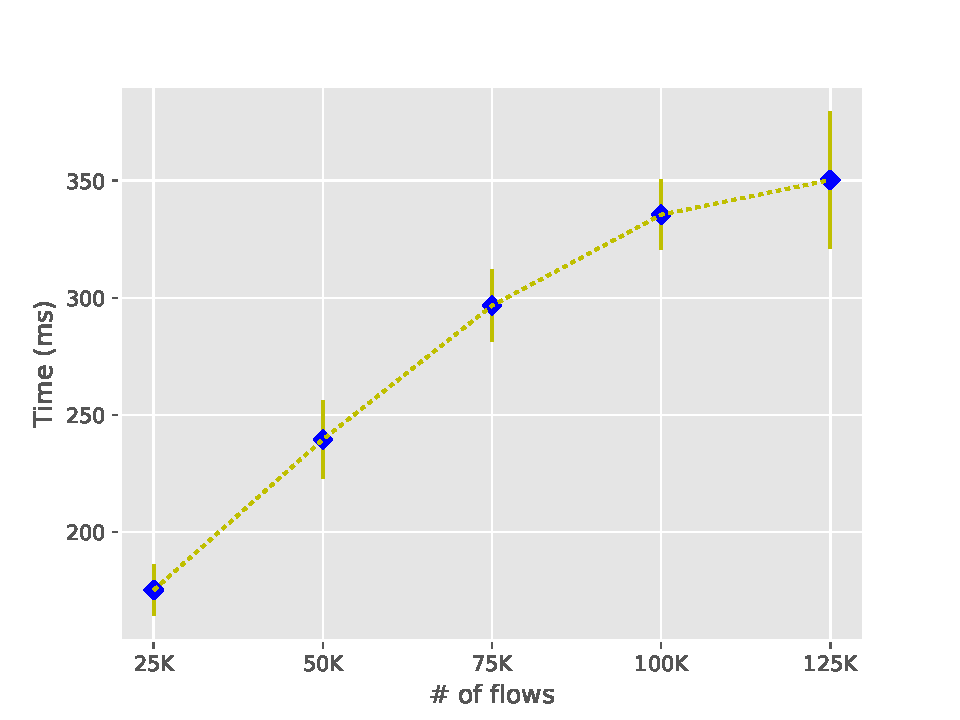
\includegraphics[width=1.05\columnwidth]{figure/Migration.pdf}
		\caption{}\label{fig:tot-mig} \end{subfigure}\hfill
	 \begin{subfigure}[t]{0.49\linewidth}
		\centering
		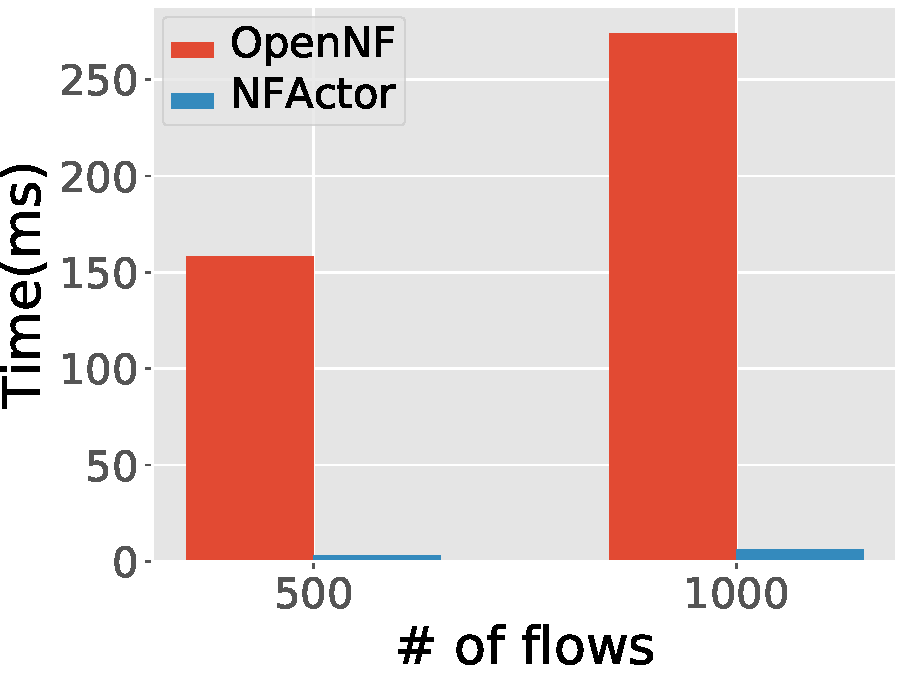
\includegraphics[width=\columnwidth]{figure/Compare.pdf}
		\caption{}\label{fig:compare-opennf}
	 \end{subfigure}
\caption{ Time consumption for flow migration.} %(a) The total time to migrate different numbers of flows concurrently on three runtimes. (b) The flow migration performance of NFActor. Each flow in NFActor runtime goes through the same service chain as in Figure \ref{fig:tot-mig}. OpenNF controlls PRADS asset monitors. The flow packet rate is 20pps.}
\label{fig:mig-perf}
\end{figure}


To inspect performance of flow migration in \nfactor, we show time taken for migrating large numbers of flows. We run three runtimes on each server, configured to run service chain ``firewall $\rightarrow$ http parser $\rightarrow$ load balancer''. The traffic generator produces flows of rate $20pps$ each, and virtual switches dispatch flows evenly to runtimes on one of the servers. %, therefore each runtime on the first server processes approximately the same number of flows.
 After the traffic stabilizes, the coordinator asks all runtimes on that server to migrate all their flows to three runtimes on another server, concurrently.

We vary the number of flows injected to each runtime and show in Fig.~\ref{fig:tot-mig} completion time for migrating all flows from a runtime, averaged over all three runtimes. We can see that it takes $350$ms for migrating about $125000$ flows (with 2.5Mpps packet processing throughput). %\chuan{complete xx. how do you come up with `even when migrating more than 300000 flows, with 6Mpps processing throughput'?}.
The time only increases sublinearly with the increase of flows. Considering the migration is concurrently carried out among three pairs of runtimes, the results show good efficiency of our distributed flow migration and the following design:
%The key reason that~\nfactor is able to achieve such a good flow migration performance is because
(i) flow states are directly copied into remote actor messages without the need for serialization and deserialization, and (ii) remote actor messages are directly encapsulated in L2 network packets and transmitted using DPDK. %with high-performance packet I/O.

We also observe zero packet loss throughout the experiment. %keep the number of lost packet due to migration target buffer overflow or packet reordering. Throughout the entire experiment, this number is zero.
 This shows that the collective buffer of a capacity of 4096 packets (for all migration target actors to buffer received flow packets in a runtime before the request in the 3rd request-response step is received), is sufficient even when migrating a large number of flows. %This buffer size is large enough to \chuan{justify why maintaining this buffer size per actor is reasonable}.

We also compare \nfactor~with OpenNF \cite{gember2015opennf} for flow migration. We send the same number of flows to \nfactor~runtimes and NFs controlled by OpenNF, and present the total time to migrate these flows in Fig.~\ref{fig:compare-opennf}.\footnote{We were not able to test under large numbers of flows due to unexpected failures when running OpenNF, possibly due to our lack of experience in operating its authors' program.} Flow migration in \nfactor~takes much less time. Though this may not be a very fair comparison as OpenNF uses legacy NFs while \nfactor~relies on NFs implemented following our design, we believe the results are still illustrative.

%Each flow in NFActor runtime goes through the same service chain as in Figure \ref{fig:tot-mig}. OpenNF controlls PRADS asset monitors. The flow packet rate is 20pps.

%the migration completion time of \nfactor~is more than 50\% faster than OpenNF.  This performance gain primarily comes from the simplified migration protocol design with the help of actor framework. In \nfactor, a flow migration process only involves transmitting 3 request-responses. Under light workload, the flow migration can complete within several hundreds of microseconds. Under high workload, \nfactor~runtime system controls the maximum number of concurrent migrations to control the migration workload, which may increase the migration performance as indicated in figure \ref{fig:avg-time-batch-mig}. All of these factors contribute to the improved flow migration performance of \nfactor~framework.

%three runtimes and migrate flows from one runtime on the firs

%We present the evaluation result of flow migration in this section. In order to evaluate flow migration performance, we initialize the cluster with 2 runtimes running with 2 worker threads and then generate flows to one of the runtimes. Each flow is processed by the service chain consisting of all the 3 NF modules. We generate different number of flows, each flow has the same per-flow packet rate. In order to see how the evaluation performs under different per-flow packet rate, we also tune the per-flow packet rate with 10pps, 50pps and 100pps. When all the flows arrive on the migration source runtime. The migration source runtime starts migrating all the flows to the other runtime in the cluster. We calculate the total migration time and the average per-flow migration time. In order to control the workload during the migration, the runtime only allows 1000 concurrent migrations all the time. The result of this evaluation is shown in figure \ref{fig:mig-perf}.

%We can see that as the number of migrated flows increase, the migration completion time increases almost linearly. This is because the average flow migration time remains almost a constant value and the runtime controls the maximum number of concurrent migrations. Note that when the system is not overloaded at all (100 flows), the average flow migration completion time is as small as 636us.

%When the per-flow packet rate is 100pps, the maximum number of flows that we use to evaluate the system is 6000. Continuing the evaluation with 8000 and 10000 flows just overloads the runtime as shown in figure \ref{fig:normal-performance}.

 %\begin{figure}[!t]
 %\begin{subfigure}[t]{0.49\linewidth}
%		\centering
%		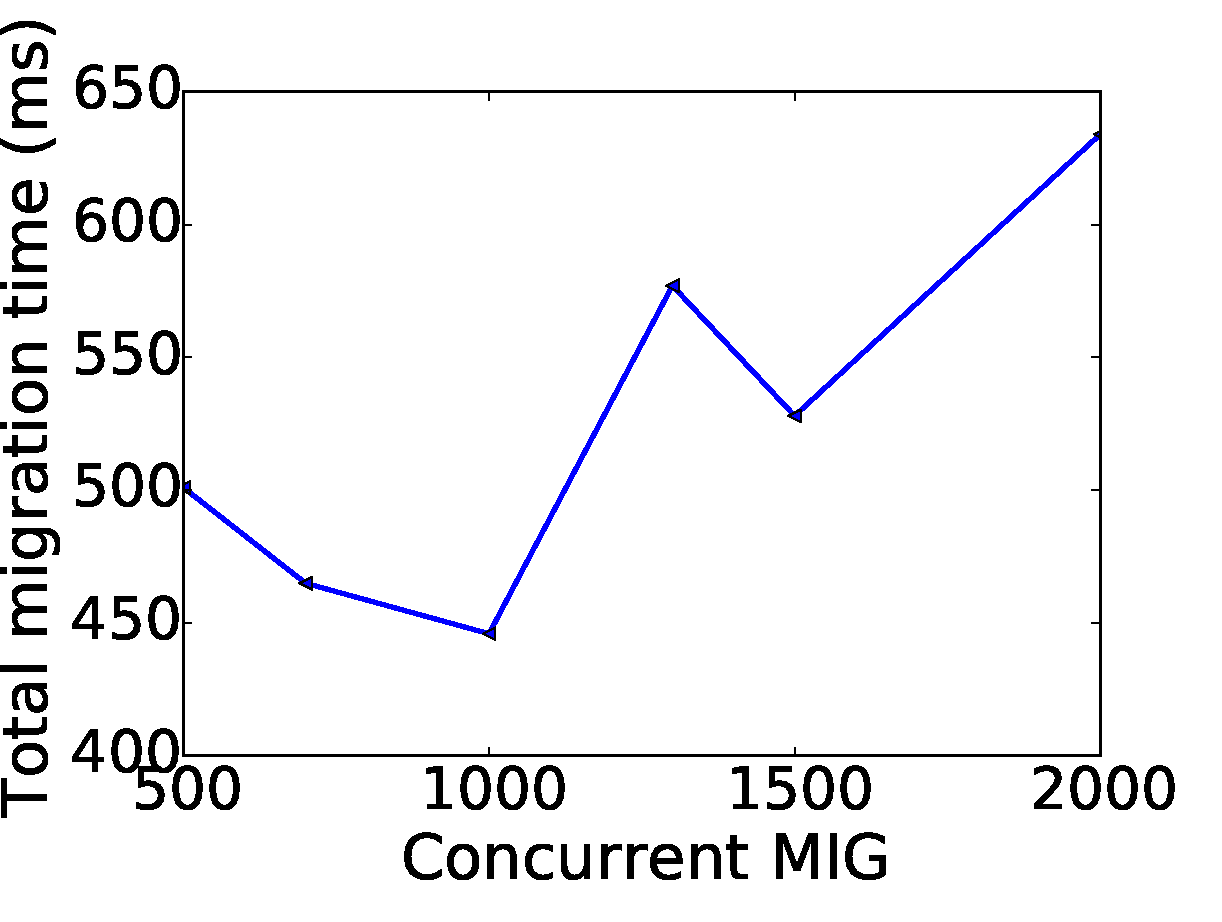
\includegraphics[width=\columnwidth]{figure/vary_batch_tot_migration_time.pdf}
%		\caption{The total time to migrate all the flows when changing the maximum concurrent migrations.}\label{fig:avg-time-batch-mig}
%	 \end{subfigure}\hfill
%	 \begin{subfigure}[t]{0.49\linewidth}
%	\centering
%		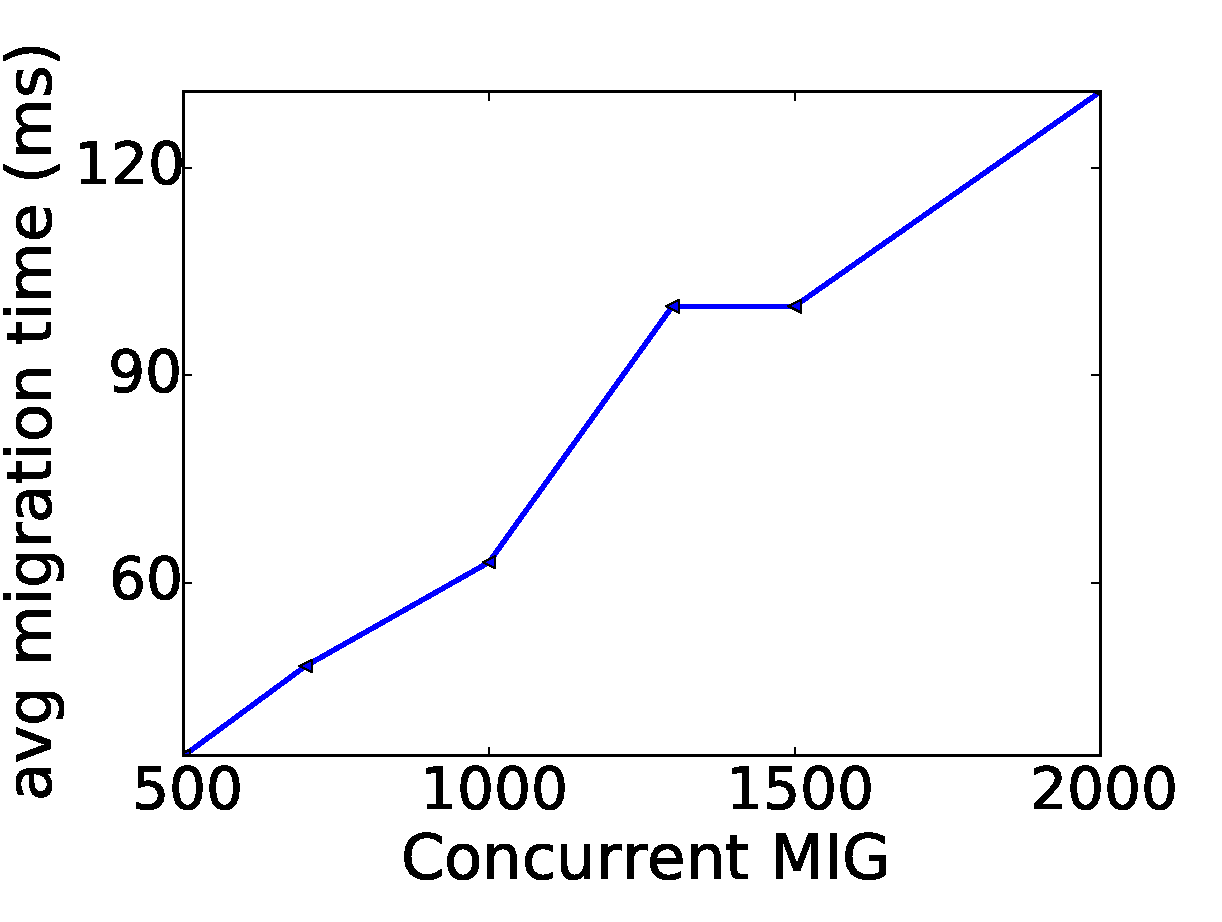
\includegraphics[width=\columnwidth]{figure/vary_batch_avg_migration_time.pdf}
%		\caption{The average flow migration time of a single flow when changing the maximum concurrent migrations.}\label{fig:avg-mig-batch} \end{subfigure}
%	\caption{The flow migration performance of \nfactor~when changing the maximum concurrent migrations.}
%\label{fig:mig-perf}
%\end{figure}

%Since we control the number of concurrent migrations, we also want to see what happens if we change the number of concurrent migrations. We generate 6000 flows, each with 50 pps per-flow packet rate, and change the the number of concurrent migrations. The result of this evaluation is shown in fig \ref{fig:mig-perf}. As we can see from fig \ref{fig:avg-mig-batch}, increasing the maximum concurrent migrations increase the average flow migration completion time. However, whether the total flow migration completion time increased depends on the total number of flows that wait to be migrated. From the result of fig \ref{fig:avg-time-mig}, the choice of 1000 concurrent migrations sits in the sweat spot and accelerates the overall migration process.

 %\begin{figure}[!t]
%		\centering
%		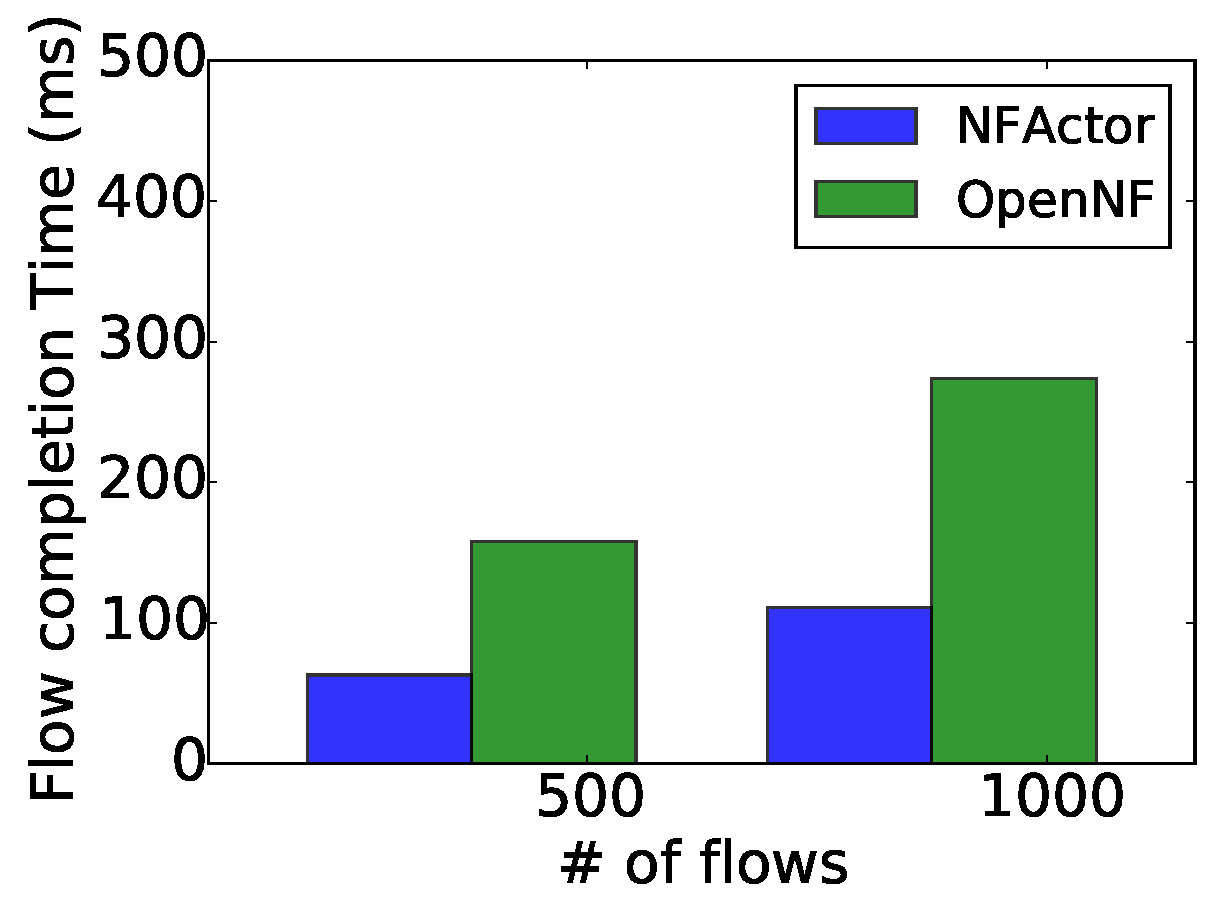
\includegraphics[width=0.6\columnwidth]{figure/opennf_nfactor_cmpFlowtime.p%df}
%		\caption{The flow migration performance of \nfactor. Each flow in \nfactor~runtime goes through the service chain consisting of the 3 customzied NF modules. OpenNF controlls PRADS asset monitors.}
%\label{fig:compare-opennf}
%\end{figure}

%Finally, we compare the flow migration performance of \nfactor~against OpenNF \cite{gember2015opennf}. We generate the same number of flows to both \nfactor~runtimes and NFs controlled by OpenNF and calculate the total time to migrate these flows. The evaluation result is shown in figure \ref{fig:compare-opennf}. Under both settings, the migration completion time of \nfactor~is more than 50\% faster than OpenNF.  This performance gain primarily comes from the simplified migration protocol design with the help of actor framework. In \nfactor, a flow migration process only involves transmitting 3 request-responses. Under light workload, the flow migration can complete within several hundreds of microseconds. Under high workload, \nfactor~runtime system controls the maximum number of concurrent migrations to control the migration workload, which may increase the migration performance as indicated in figure \ref{fig:avg-time-batch-mig}. All of these factors contribute to the improved flow migration performance of \nfactor~framework.

\subsection{Throughput during Dynamic Scaling}

%\begin{figure}[!t]
%	\centering
%	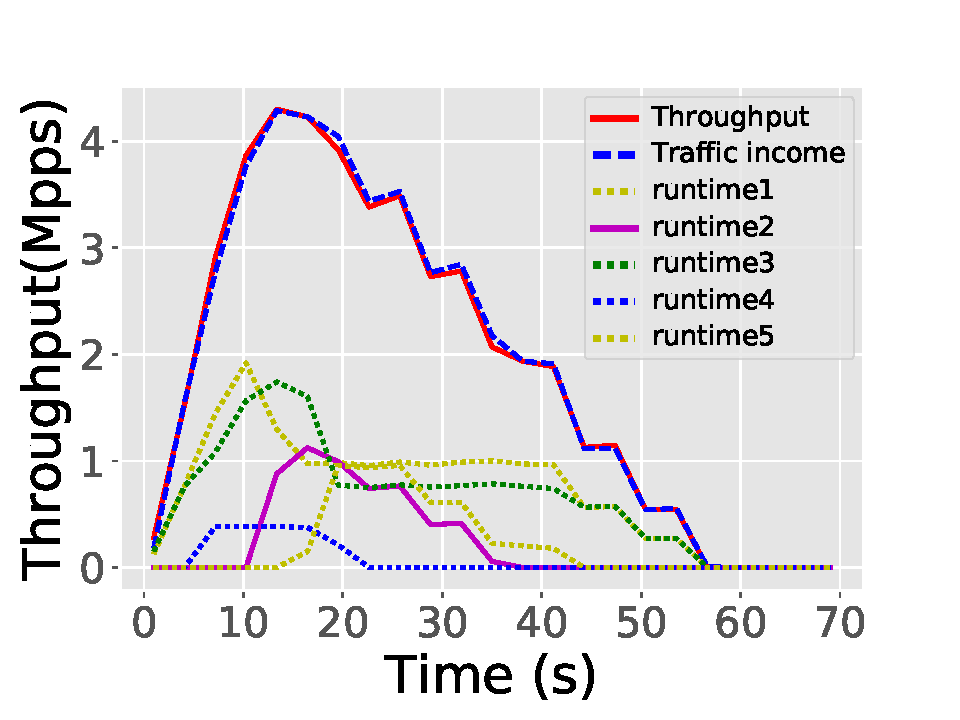
\includegraphics[width=\columnwidth]{figure/Scale.pdf}
%	\caption{Throughput during dynamic scaling.}
%\label{fig:normal-case-scale}
%\end{figure}

\begin{figure*}[!t]
\captionsetup{width=0.3\textwidth}
\begin{center}
\begin{minipage}[t]{0.355\linewidth}
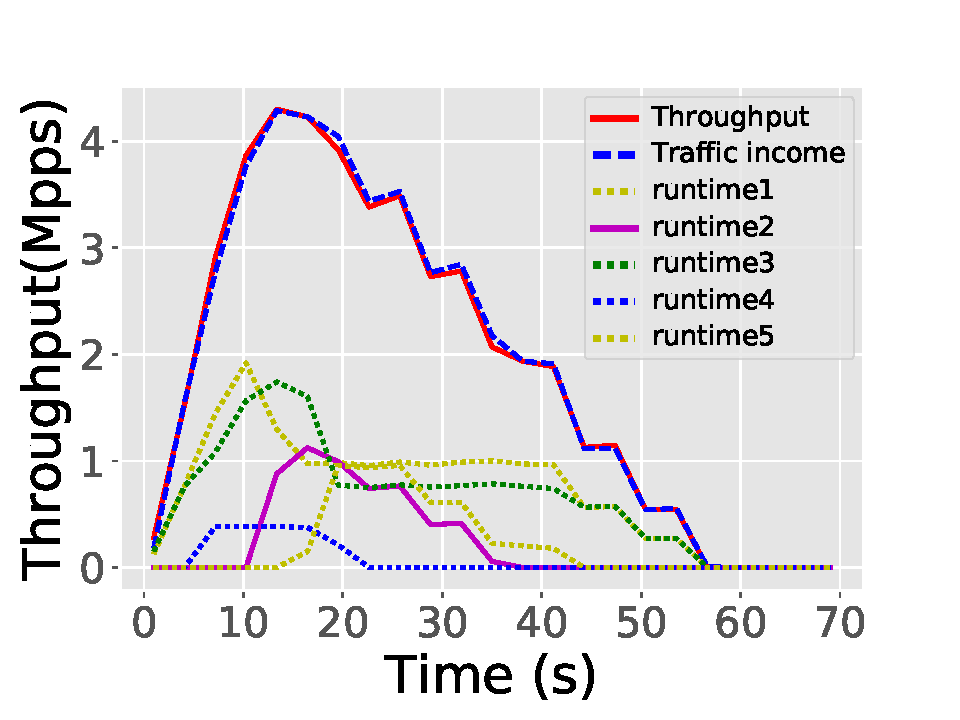
\includegraphics[width=1\textwidth]{figure/Scale.pdf}
	\caption{Throughput during dynamic scaling.}
\label{fig:normal-case-scale}
\end{minipage}
\hfill
\begin{minipage}[t]{0.615\linewidth}
 \begin{subfigure}[t]{0.48\linewidth}
		\centering
		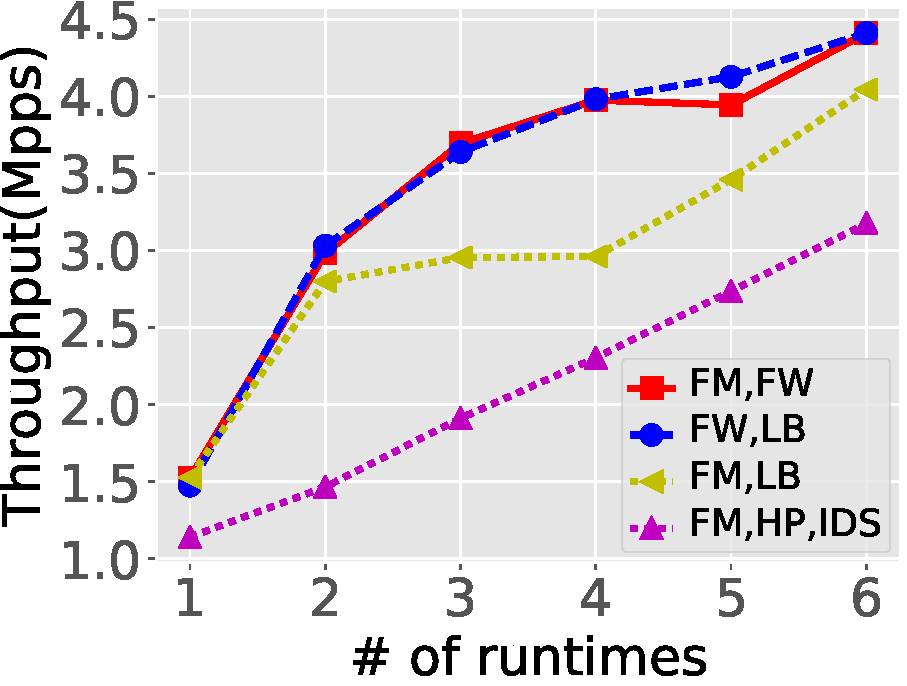
\includegraphics[width=\columnwidth]{figure/ReplicaTP.pdf}
		%\caption{The packet throughput of a \nfactor~cluster when replication is enabled. }
		\caption{}\label{fig:rep-scale}
	 \end{subfigure}\hfill
	 \begin{subfigure}[t]{0.49\linewidth}
	\centering
		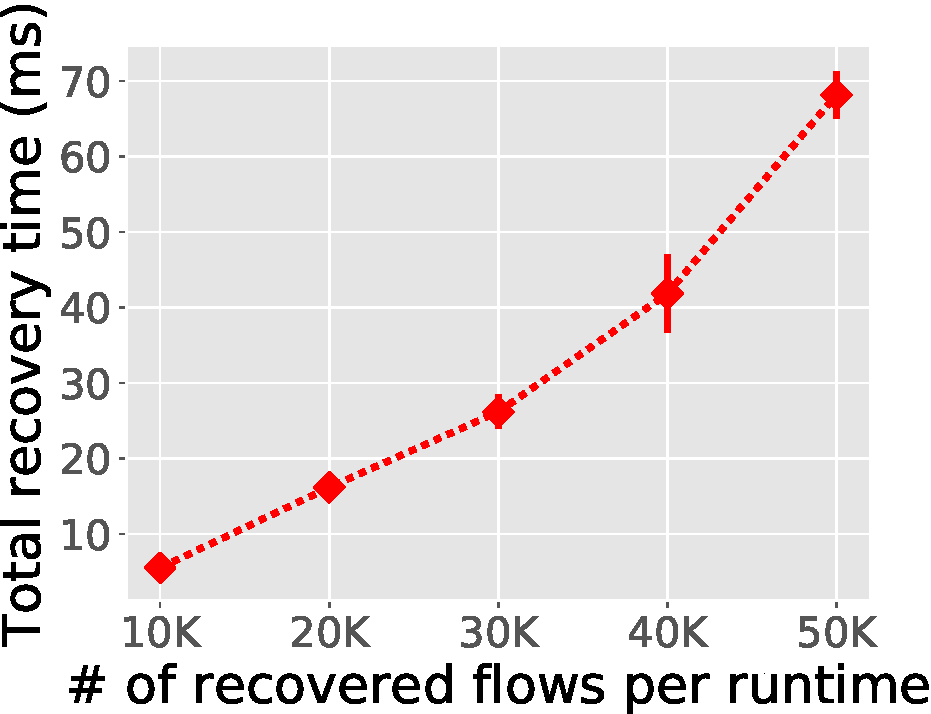
\includegraphics[width=1\columnwidth]{figure/Recover.pdf}
		%\caption{The recovery time of three failed runtimes under different settings. The tuple on the $x$ axis represents the number of the runtime used in the evaluation and the total input packet rate. }
		\caption{}\label{fig:rep-recovery} \end{subfigure}
	\caption{Performance of flow migration}
\label{fig:rep-perf}
\end{minipage}
\end{center}
\vspace{-5mm}
\end{figure*}


We further evaluate performance of dynamic scaling mechanism in \nfactor. The traffic generator produces a varying number of flows overtime. Each flow has a rate of 20pps, lasting 60 seconds. The runtimes are configured with service chain ``firewall $\rightarrow$ HTTP parser $\rightarrow$ IDS''. Fig.~\ref{fig:normal-case-eval} shows that the cluster is scaled up to 6 runtimes to handle the peak rate. We observe that whenever a runtime is overloaded (runtime 1 and runtime 4), our mechanism promptly resolves the hotspot (considering each flow lasts 60s). %, without the efficient and distributed flow migration. ~\nfactor would not be able to achieve this, but continue to be overloaded for a long period of time, resulting in severe performance drop.

We further observe in our experiment that the CPU usage of the coordinator remains under 5\%, due to its lightweight design.


\subsection{Performance of Flow Replication}
\label{sec:rp}

\begin{comment}
 \begin{figure}[!t]
 \begin{subfigure}[t]{0.49\linewidth}
		\centering
		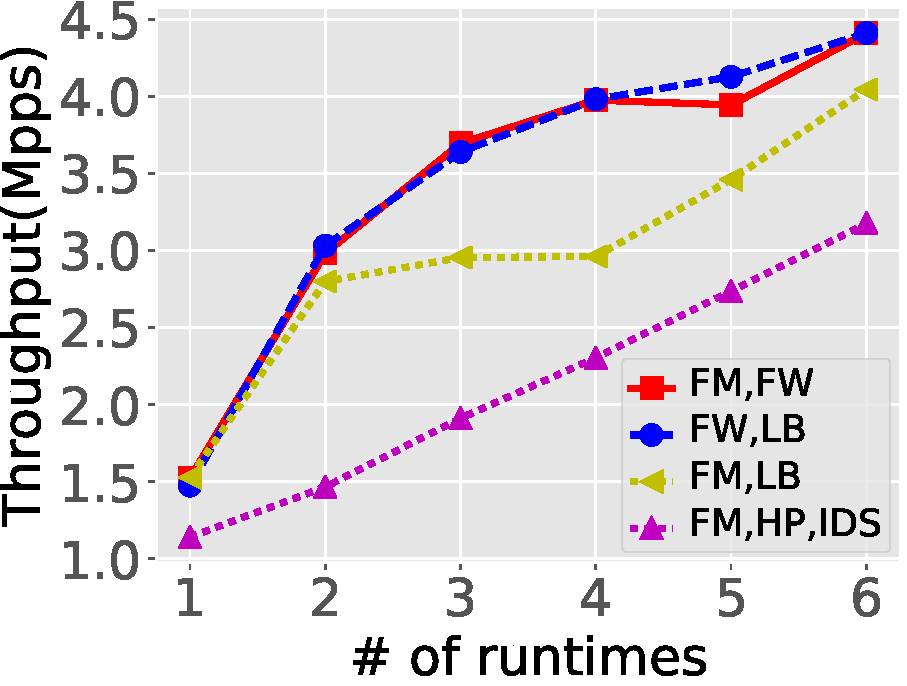
\includegraphics[width=\columnwidth]{figure/ReplicaTP.pdf}
		%\caption{The packet throughput of a \nfactor~cluster when replication is enabled. }
		\caption{}\label{fig:rep-scale}
	 \end{subfigure}\hfill
	 \begin{subfigure}[t]{0.49\linewidth}
	\centering
		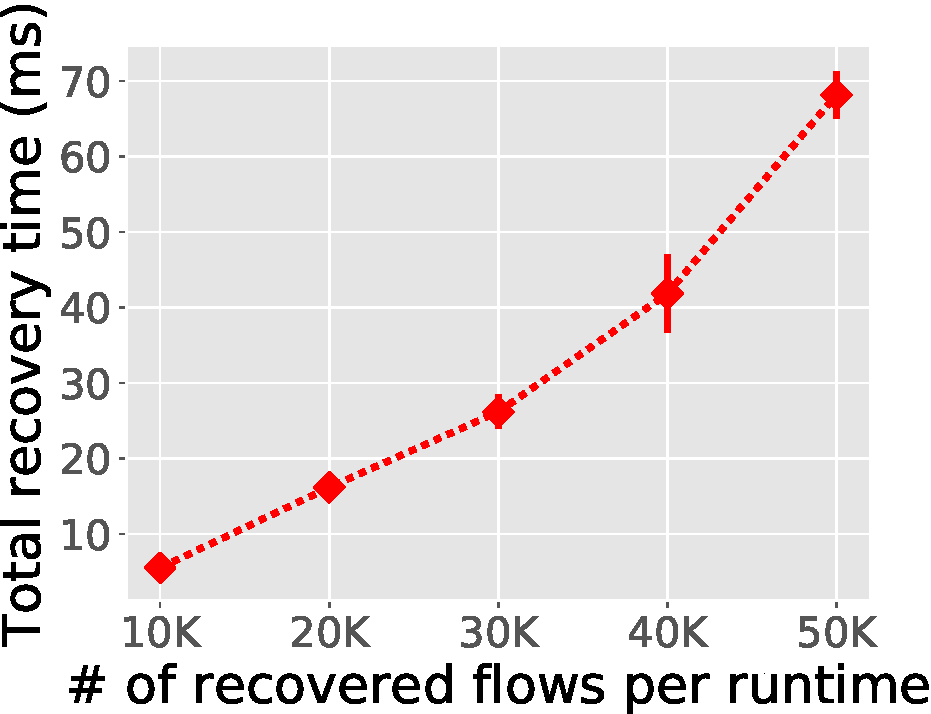
\includegraphics[width=\columnwidth]{figure/Recover.pdf}
		%\caption{The recovery time of three failed runtimes under different settings. The tuple on the $x$ axis represents the number of the runtime used in the evaluation and the total input packet rate. }
		\caption{}\label{fig:rep-recovery} \end{subfigure}
	\caption{Performance of flow migration}
\label{fig:rep-perf}
\end{figure}
\end{comment}
%\chuan{Fig.~\ref{fig:rep-scale}: better to make the service chains in Fig. \ref{fig:normal-case-eval} and this figure the same, such that readers can compare the difference with and without flow replication}


%both in terms of overall packet processing throughput achieved during flow replication and the recovery time when a runtime fails.  Therefore we set up several runtimes on a server, configure each of these runtimes with a dedicated replica runtime on anther server.

We next enable flow replication in \nfactor. The traffic generator produces 300K flows with a flow rate of 30pps.  % to generate traffic to the runtimes being replicated, and
Four different service chains are used in this experiment.
Three runtimes are running on each server.
%calculate the accumulated packet throughput from the replica.

Fig.~\ref{fig:rep-scale} shows that with the increase of runtimes deployed for each service chain, the packet processing throughput from runtimes running each service chain increases, but is always lower than the throughput if no flow replication is in place. %. For runtimes running service chains consisting of lightweight NFs (\eg, flow monitor, firewall and load-balancer), the overall throughput gradually increases to around 4Mpps
% 9Mpps. %\chuan{give the largest throughput if not doing flow replication}.
At the peak througput, the bandwidth on the L2 network has been saturated and becomes the bottleneck. This is because for each input packet, an additional packet is transmitted from the original runtime to the replication target runtime, %at least two output packets,
 containing the flow states and the output packet processed by the flow actor. These packets consume additional bandwidth in the system. %Being transmitted through reliably to the remote side, these packets are also appended with a header (the average size is 25bytes for each packet), further increase the bandwidth usage.
 We believe such additional bandwidth consumption is unavoidable if to ensure the % that our flow replication scheme remains its applicability because it achieves the
 output-commit property. To mitigate this issue, a flow actor can replicate its flow states after it has processed multiple packets, at the cost of weaker flow state consistency. %is weaker,~\nfactor could be easily adapted to use a light-weight replication scheme, that replicates the the flow state after it has processed multiple packets, to increase the throughput.

The biggest advantage brought by \nfactor's flow replication is the fast recovery time in case of failures. %Following the settings as in Figure~\ref{fig:rep-scale},
We emulate a server crash by shutting down the server, and recover flows processed by failed runtimes on their replicas on other servers. Fig.~\ref{fig:rep-perf} shows that 50000 flows can be recovered within tens of milliseconds. This is because flow recovery in \nfactor~is extremely lightweight, involving only one request-response pass between the replica runtime and the virtual switch. % for each replicated flow actor.

We do not show results evaluating failure resilience of the coordinator and the virtual switches, since their handling in cases of failures is mostly standard as in the literature.

%To evaluate~\nfactor's flow replication, we configure the virtual switch to generate output packets to runtimes on the first server. For each runtime on the first server, we configure a replica runtime on the second server, and let each runtime replicate its flows to the corresponding replica runtime. We calculate the cumulative packet processing throughput during flow replication. The result is shown in Figure~\ref{fig:rep-scale}. We can see that the scalability during flow replication is not as good as the result achieved when replication is disabled. The replication throughput can achieve an almost linear scalability when there are smaller than four runtimes running in a single server, but the scalability starts to degrade when more runtimes are used. The primary reason is because the bandwidth consumption on the L2 network is way higher than normal case evaluation. To ensure output-commit property, for each input packet, the runtime generates at least two output packets, containing the flow state and the output packet processed by the flow actors.

%~\nfactor replicates the flow state for each processed packet using a reliable message passing module. The number of transmitted packets by the reliable message passing module is actually two times the number of the input packets. To reliably transmit flow state and the processed packet, the runtime also needs to add a header for each remote actor message, which is 52 byte long in our implementation. All these reasons contribute to a much larger bandwidth that are actually delivered over the network, which may result in potential packet drops.

%In this section, we present the flow replication evaluation result. In our evaluation, the actor creates a flow snapshot for every 10 flow packets that it has processed. Then it sends the flow state snapshot to the replica storage. In this evaluation, we first generate flows to the \nfactor~cluster to test the maximum throughput of a \nfactor~cluster when enabling replication. Then we calculate the recovery time of failed \nfactor~runtime. The recovery time is the from time that the controller detects a \nfactor~runtime failure, to the time that the recovered \nfactor~finishes replaying all of its replicas and responds to the controller to rejoin the cluster. Through out this evaluation, the runtime uses the service chain consisting of the 3 NF modules to process the flow. The result of the evaluation is shown in figure \ref{fig:rep-perf}.

%In figure \ref{fig:rep-scale}, we can see that there is an obvious overhead to enable replication on \nfactor~runtimes. The overall throughput when replication is enabled drops around 60\%. This is due to the large amount of replication messages that are exchanged during the replication process. Internally, the replication messages are sent over Linux kernel networking stack, which involves data copy and context switching, thus increasing the performance overhead of using replication. However, the overall throughput when replication is enabled could scale to 850K pps when 4 runtimes are used, which is enough to use in some restricted settings.

%Finally, figure \ref{fig:rep-recovery} shows the recovery time of \nfactor~runtime when replication is enabled. We found that the recovery time remains a consistent value of 3.3s, no matter how many runtimes are used or how large the input traffic is. The reason of this consistent recovery time is that the \nfactor~runtime maintains one replica on every other \nfactor~runtimes in the cluster. During recovery, several recovery threads are launched to fetch only one replica from another runtime. Then each recovery thread independently recovers actors by replaying its own replica. In this way, the recovery process is fully distributed and scales well as the number of replica increases. Note is that the average time it takes for a recovered runtime to fetch all the replicas and recover all of its actors is only 1.2s. So actually around 2.1s is spent in container creation and connection establishment.


\subsection{Other Applications}
\label{sec:applications}



In addition, we build two applications based on \nfactor, which exploit its lightweight, distributed flow migration capability to achieve useful functionalities. %, including live NF update, reduce output bandwidth for deduplication NF and ensure reliable and safe MPTCP processing. We evaluate and demonstrate these new applications in our evaluation.

\vspace{1mm}
\noindent\textbf{Live NF update.} %NF often needs to be updated (\eg, software version, important NF configuration files), existing systems would typically migrate flows away, stop the NF and then relaunching it.
 \nfactor~can achieve dynamic NF update (\eg, software version, important NF configuration files) without interfering active flows, by dynamically migrating the flows out to a replica runtime, performing update and migrating the flows back. Fig.~\ref{fig:dynamic-update} illustrates the throughput of a runtime running a firewall NF, during dynamic update of its firewall rule. No active flows are dropped during the update with \nfactor, while significant throughput drop occurs if shutting down the firewall for its update.

\vspace{1mm}
\noindent\textbf{MPTCP sub-flow processing.} When an MPTCP \cite{wischik2011design} flow traverses an NFV system, its sub-flows may be sent to different NF instances for processing. Some network functions require all subflows to be processed by the same instance, \eg, IDS. % requires that all subflows of the same MPTCP flow to be examined by the same IDS instance to detect potential netowrk attacks.
In \nfactor, we can add an MPTCP sub-flow detection function to each flow actor, such that when the flow actor processes the first packet of a flow, it can check whether it belongs to an MPTCP flow. If so, the flow actor performs a consistent hashing using the MPTCP header to decide a migration target runtime in the cluster, and migrates the flow to the target. In this way, different sub-flows belonging to the same MPTCP flow can be processed by the same flow actor. This is hard to be achieved in the existing NFV systems without significant central coordination. %, since flows can not initiate active migration request by themselves.

In the experiment of Fig.~\ref{fig:mptcp}, we inject a total number of about 320K MPTCP flows to 3 runtimes. With subflow detection enabled, the total number of correctly processed MPTCP flows is always the same as the number of input flows, \ie, those whose subflows are all processed by the same runtime. Without this detection, most of the subflows are processed by different runtimes. % therefore only a small amount of MPTCP flows are correctly processed.

\begin{figure}[!t]
\begin{subfigure}[t]{\linewidth}
   \centering
   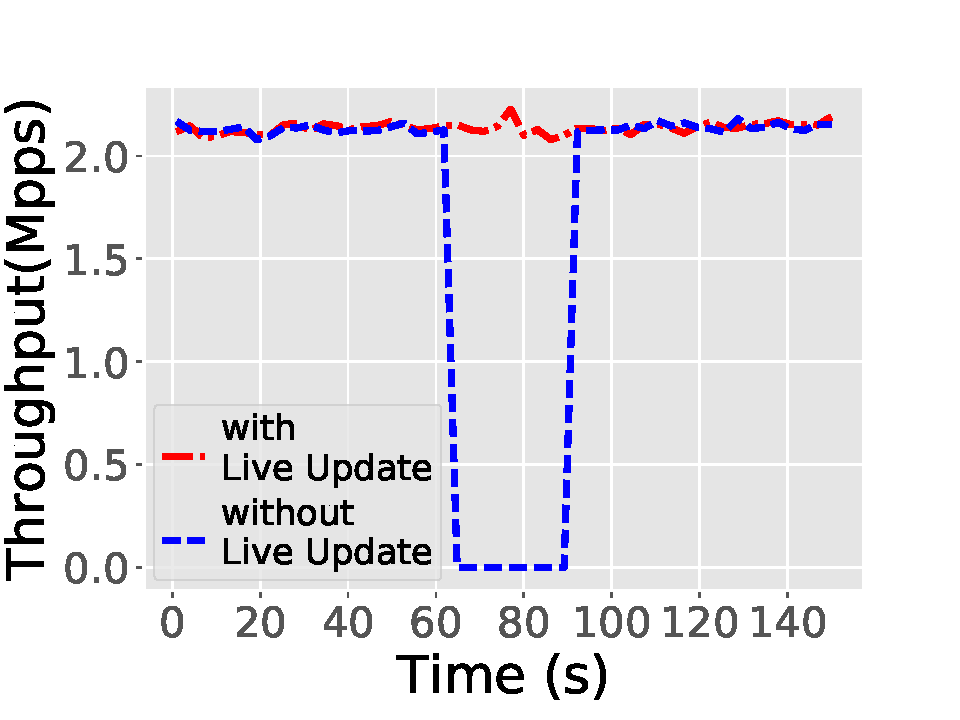
\includegraphics[width=0.7\columnwidth]{figure/Dynamic.pdf}
   %\caption{The packet processing throughput when dynamically update the firewall rule of a runtime configured with firewall NF. }
   \caption{}\label{fig:dynamic-update}
  \end{subfigure}\hfill
  \begin{subfigure}[t]{\linewidth}
 \centering
   \includegraphics[width=0.75\columnwidth]{figure/MPTCP.pdf}
   %\caption{Total number of correctly processed MPTCP flows by three runtimes when MPTCP detection is enabled on runtimes or disabled on runtimes.}
   \vspace{-2mm}
   \caption{}\label{fig:mptcp} \end{subfigure}%\hfill
  %\begin{subfigure}[t]{0.33\linewidth}
% \centering
 %  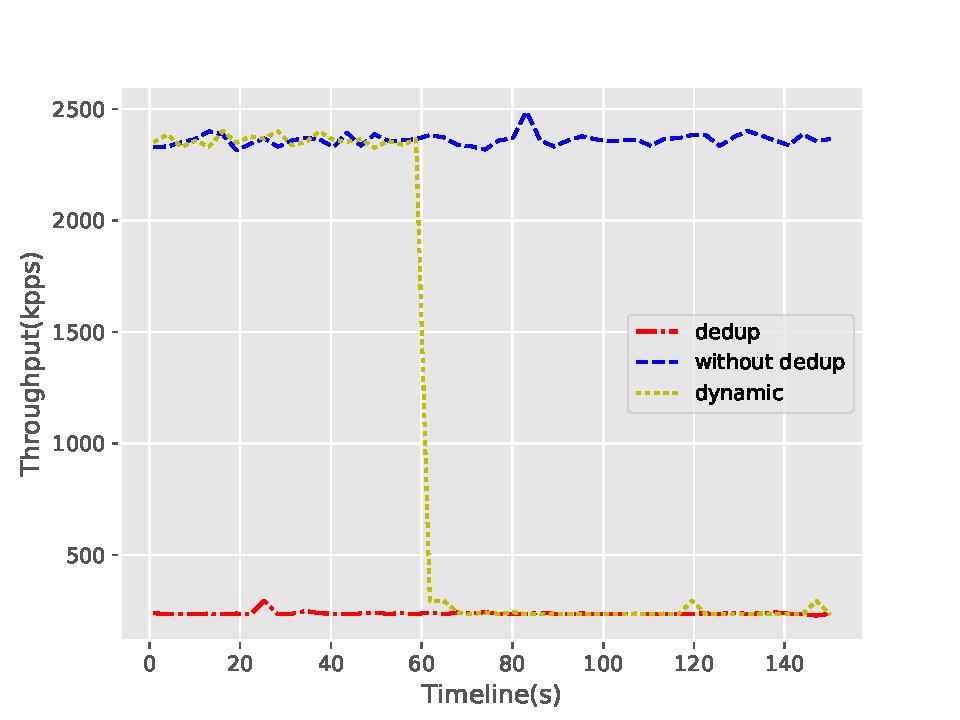
\includegraphics[width=\columnwidth]{figure/Dedup.pdf}
   %\caption{The output throughput of three runtimes when deduplication is disabled, enabled or enabled half way. }
 %  \caption{}\label{fig:deduplication} \end{subfigure}
 \vspace{-2mm}
 \caption{New applications enabled with distributed flow migration capability of \nfactor.}
\label{fig:rep-perf}
\end{figure}

%The final application is similar with MPTCP application, which reduces the output bandwidth for deduplication.

%\vspace{1mm}
%\noindent\textbf{Flow Deduplication.} Flow deduplication, as an important functionality of WAN optimizers \cite{anand2010cheap}, is useful for reducing bandwidth consumption due to transfer redundant data across different flows. \nfactor~can efficiently support flow deduplication: when a runtime receives a flow, it checks for duplicated content contained in the flow packet by performing a consistent hash over the entire packet content. \chuan{how does it check duplicated content among different flows received on different runtimes? otherwise, duplicate with whom?}.
%If duplication identified, the flow actor initiates a migration to move the flow to a specific runtime, as indicated by the hash value of the packet content. In this way, duplicated flows can be processed on the same runtime, eliminating redundant processing and bandwidth consumption. When the duplicated flows arrive on the same runtime, before the packets are sent out from the runtime, we use the liason actor to intercept duplicated packet, and only generate an output data packet for every 10 duplicated packet it receives. The output data packet is packed with useful information (\ie packet header of dupliated packet plus an identifier for identifying the duplicated content), so that the receiver on the other end could reconstruct all the original duplicated packets.
%Figure~\ref{fig:deduplication} illustrates deduplication performance. We can see that deduplication decreases the number of output packets by around 90\% through effective deduplication.
 %actors send the output packet out, the runtime intercepts duplicated content,  \chuan{why processing duplicated flows on the same runtime can reduce output bandwidth? Are they processed by the same flow actor? what if the flows are partially duplicated but not entirely?}. This is hard to be achieved in existing NFV systems because xxx \chuan{give the reason}.

%\section{Discussions}
\label{sec:discussion}

We point out a few limitations of \nfactor, and intriguing future directions.

%To achieve transparent resilience,
To achieve clean separation between flow state and NF core logic, \nfactor~requires NFs rewritten using a set of APIs (Sec.~\ref{sec:NFAPIs}). With the advance of NFV, more and more new NFs will be created. If using the actor model for constructing NFV systems is accepted by the community, we believe it feasible to create new NFs following our design. %, that processes flows based on flow state could achieve transparent resilient if they are implemented using~\nfactor.

Though focusing on stateful NFs, %Due to the use of lightweight actors, 
\nfactor~can handle non-stateful NFs as well with ease. Non-stateful NFs can also benefit from the fast, distributed flow migration, as it eliminates potential packet re-ordering caused by directly changing the path of a flow.
%\chuan{briefly discuss what if nfactor is used to handle non-stateful NFs, short flows}

%Even though~\nfactor provides transparent resilience for stateful NFs,
\nfactor~focuses on handling per-flow state, consisting of states of NFs along the flow path. The current \nfactor~framework does not correctly handle shared states, \ie, the states shared by a bunch of flows \cite{bro}. The reason is that %Even though the NF API in~\nfactor achieves a clean separation between per-flow state and NF processing logic,
our current NF API design does not achieve correct separation of shared states. Migrating and replicating flows that share states with other flows may lead to un-predictable errors. A potential solution is to implement a handler on flow actor that explicitly deals with state inconsistency during flow migration and replication. We leave this to our future work.

In addition, \nfactor~may incorrectly handle flows with packet encapsulation. \nfactor~uses the 5-tuple to differentiate flows. Different flows may share the same 5-tuple if their original flow packets are encapsulated using similar headers. This is common for flows sent over the same VxLAN tunnel. In that case, those flows are handled by the same flow actor using the same service chain, potentially incorrect. If we know what kind of encapsulation the input flows use, we may add a decapsulation function in the virtual switch to correctly extract different flows. This will also be further investigated in our future work.

\section{Background and Related Work}
\label{sec:relatedwork}



\subsection{Network Function Virtualization}

NFV was introduced by a 2012 white paper \cite{nfv_whitepaper} by telecommunication operators that propose running virtualized network functions on commodity hardware. Since then, a broad range of NFV studies has been seen in the literature, including bridging the gap between specialized hardware and network functions \cite{hwang2015netvm, Han:EECS-2015-155, martins2014clickos, 199352}, scaling and managing NFV systems \cite{gember2012stratos, palkar2015e2}, flow migration among different NF instances \cite{rajagopalan2013split, khalid2016paving, gember2015opennf}, NF replication \cite{rajagopalan2013pico, sherry2015rollback}, and traffic steering \cite{simplifying}. %None of these systems provide a uniform runtime platform to execute network functions.
In these systems, the NF instances are created as software modules running on standard VMs or containers. \nfactor~customizes a uniform runtime platform to run network functions, which enables transparent resilience support for all network functions/service chains in the runtimes. In addition, a dedicated service chain instance is provisioned for each flow, enabled by the actor framework, achieving failure tolerance and high packet processing throughput with ease. Even though modular design introduced by ClickOS  \cite{martins2014clickos} %\cite{kohler2000click}
 simplifies the way how NFs are constructed, advanced control functionalities, \eg, that to enable flow migration, are still not easy to be integrated in NFs following the design. %nowadays there are new demands for NFV system, which require advanced control functionality to be integrated even into the NF softwares.

%Among the advanced control functionality, flow migration and fault tolerance are definitely the two of the most important features.
%\chuan{cite as many as possible the systems you mentioned in the introduction in the following paragraph, E2 \cite{palkar2015e2}, OpenBox \cite{OpenBox}, CoMb \cite{sekar2012design}, xOMB \cite{anderson2012xomb}, Stratos \cite{gember2012stratos}, OpenNetVM \cite{hwang2015netvm, zhang2016opennetvm}, ClickOS \cite{martins2014clickos}; discuss more of the recent work \cite{StandardAPI} and \cite{OpenBox}}

A number of NFV systems \cite{palkar2015e2, OpenBox, sekar2012design, anderson2012xomb, hwang2015netvm, zhang2016opennetvm, martins2014clickos, zhang2016flurries} have been proposed to manage NF service chains or graphs in an effective and high-performance way. Among these work, Flurries \cite{zhang2016flurries} proposes to do fine-grained per-flow NF processing, and is able to dynamically assign a flow to a light-weight NF. While sharing some similarities,~\nfactor~focuses on applying actor model to perform micro service chain processing for each flow, and uses actor model to provide transparent resilience. It is possible to expand the service chain processing in~\nfactor~to service graph processing as in E2 \cite{palkar2015e2} and OpenBox \cite{OpenBox} because~\nfactor~uses a run-to-completion scheduling strategy to process flow packets. But~\nfactor~sticks to the service chain processing as it still represents the mainstream processing method \cite{hwang2015netvm, martins2014clickos}.

%Even though the service chain concept has been expanded to service graphs in E2 \cite{palkar2015e2} and OpenBox \cite{OpenBox}, \nfactor uses the traditional service chain to process a flow as it still represents the mainstream processing method \cite{hwang2015netvm, martins2014clickos}.

To achieve flow migration, existing work such as OpenNF \cite{gember2015opennf} require direct modification of the core processing logic of NF software, which is tedious and difficult to achieve. In addition, existing NFV management \cite{rajagopalan2013split} \cite{gember2015opennf} systems % \chuan{add citation}
mostly rely on a centralized SDN controllers to carry out the flow migration protocol, involving non-negligible message passing overhead that lowers packet processing speed of the system.
%Finally, the migration process is fully controlled by a  centralized SDN controller, which may not be scalable if there are many NF instances that need flow migration service.
\nfactor~overcomes these issues using a clean separation between NF processing logic and resilience support functionalities, as well as a system design based on the distributed actor framework. The actors can be migrated by communicating among themselves without the coordination from a centralized controller. A fast virtual switch is designed to achieve the functionality of a dedicated SDN switch. Only 3 rounds of request-response are needed for achieving flow migration, based on the actor framework and the customized virtual switch, enabling fast flow migration and high packet processing throughput.

Flow replication usually involves check-pointing the entire process image \ac{ runing the NF software} %\chuan{clarify what process image this is referring to, NF process?}
and creating a replica for the created process image \cite{sherry2015rollback} \cite{rajagopalan2013pico}. The checkpointing method, such as the one used by \cite{sherry2015rollback}, may require temporary pause of an NF process, leading to flow packet losses. %\chuan{this claim does not appear to be rigorous: does all checkingpointing require pausing a process? double check and revise}.
\nfactor~is able to checkpoint all states of a flow in a lightweight fashion without introducing large delay, due to that the clean separation between NF processing logic and NF flow state enables the actor to directly store all the flow states of the service chain and transmit the flow states at any time without interfering the normal execution of the NF%\chuan{briefly describe how \nfactor can achieve this}
, enabling transparent replication of NFs and service chains.  Existing work \cite{sherry2015rollback} rely on automated tools to extract important state variables for replicating, which \ac{relies on static program analysis technique and may not accurately extract all the important state variables if the NF program is complicated and uses a new architecture}.% \chuan{explain why these tools are not ideal}.

%A NFV system \cite{nfv-white-paper} typically consists of a controller and many VNF instances. Each VNF instance is a virtualized device running NF software. VNF instances are connected into service chains, implementing certain network services, \eg, access service. Packets of a network flow go through the NF instances in a service chain in order before reaching the destination.

%A VNF instance constantly polls a network interface card (NIC) for packets. Using traditional kernel network stack incurs high context switching overhead \cite{martins2014clickos} and greatly compromise the packet processing throughput. To speed things up, hypervisors usually map the memory holding packet buffers directly into the address space of the VNF instances with the help of Intel DPDK\cite{dpdk} or netmap \cite{netmap}. VNF instances then directly fetch packets from the mapped memory area, avoiding expensive context switches. Recent NFV systems \cite{palkar2015e2, Han:EECS-2015-155, sherry2015rollback, martins2014clickos, hwang2015netvm} are all built using similar techniques.


%Even though using DPDK and netmap to improve the performance of packet processing has become a new trend. Existing flow management systems are still using kernel networking stack to implement the communication channel. On contrary, NFActor completely abandons the kernel networking stack, by constructing a reliable transmission module using DPDK. Using this reliable transmission module does not incur any context switches, thereby boosting the message throughput to 6 million messages per second in our evalution.



\subsection{Actor}

The actor programming model has been used for constructing massive, distributed systems \cite{actor-wiki, akka, newell2016optimizing, AnalysisActor}. Each actor is an independent execution unit, which can be viewed as a logical thread. In the simplest form, an actor contains an internal actor state (\eg, statistic counter, \ac{number of the out-going request} %\chuan{not intuitive why an actor's state can be status of peer actors; change to another example}
), a mailbox for accepting incoming messages and several message handler functions. An actor can process incoming messages using its message handlers, send messages to other actors through the built-in message passing channel, and create new actors. \ac{Actors are well suited to implement state machine, that modify its internal state based on the received message, therefore facilitates distributed protocol implementation.} %\chuan{explain how the actor model facilitates `distributed' protocol implementation}
In an actor system, actors are asynchronous entities that can receive and send messages as if they are running \ac{in their own threads, simplifying programmability of actors and eliminating potential race conditions which may cause the program to crash.}
%\chuan{not clear what it implies by `running in a dedicated process' - clarify what benefits it brings}.
The actors usually run on a powerful runtime system \cite{erlang, akka, caf}, \ac{which is a uniform platform to schedule actors to execute}
%\chuan{explain what runtime means here}
, enabling them to achieve network transparency, \ac{as actors could transparently communicate with remote actors running on different runtimes as they are all running on the same runtime.}
%\chuan{clarify what `network transparency' means here}.
%\chuan{discuss more how the actor model provides a natural and unified way for migrating/replicating actors}.
\ac{An actor could launch a remote actor and communicates with the remote actor to migrate/replicate all of its internal state. The remote actor could directly substitute the identity of the original actor whenever necessary. Therefore actor model provides a natural and unified way for migrating/replicating actors.}

The actor model is a natural fit when building distributed NFV systems. We can create one actor as one flow processing unit (a NF or a service chain, while the later is our design choice in \nfactor), and map flow packet processing to actor message processing. Meanwhile, flow migration and replication functions can be implemented as message handlers on the actors. Even though there exists this natural connection between the actor model and NF flow processing functions, we are not aware of any existing work that leverages the actor model to build an NFV system. % even though there is a natural connection among actor message processing and NF flow processing.
 To the best of our knowledge, we are the first to exploit the actor model in enabling resilient NFV systems and relevant applications, as well as to demonstrate the benefits of this actor-based approach.


%The actor programming model has been widely used to construct resilient distributed software \cite{erlang, akka, Orleans, caf}.

There are several popular actor frameworks, \eg, Scala Akka \cite{akka}, Erlang \cite{erlang}, Orleans \cite{Orleans} and C++ Actor Framework \cite{caf}. These frameworks have been used to build a broad range of distributed applications. %, including on-line games and e-commerce.
 For example, Blizzard (a famous PC game producer) and Groupon/Amazon/eBay (famous e-commerce websites) all use Akka in their production environment \cite{akka}. However, none of these frameworks are optimized for building NFV systems. In our initial prototype implementation, we built \nfactor on top of the C++ Actor Framework \cite{caf}, but the message-passing performance of that prototype turned out to be non-satisfactory %\chuan{describe what performance metrics you are referring to}
 , due mainly to \ac{that C++ Actor Framework uses kernel networking stack to transmit actor messages and the context switching overhead is intolerable in NFV system} \cite{martins2014clickos}. This inspires us to create a customized actor framework for \nfactor~with  significantly improved performance.

%\chuan{move the following discussion to the runtime section}
%\textbf{Lightweight Execution Context.}
%There has been a recent study on constructing lightweight execution context \cite{litton2016light} in the kernel. In this work, the authors construct a lightweight execution context is contructed by creating multiple memory mapping tables in the same process. Switching among different memory tables can be viewed as switching among different lightweight execution contexts. NFActor provides a similar execution context, not for kernel processes, but for network functions. Each actor inside \nfactor provides a lightweight execution context for processing a packet along a service chain. Being a lightweight context, the actors do not introduce too much overhead as we can see from the experiment results. On the other hand, packet processing is fully monitored by the execution context, thereby providing a transparent way for migrating and replicating flow states.

\section{Conclusion}
\label{sec:conclusion}

\nfactor~is an NFV system built using the distributed actor model, to achieve transparent resilience, high scalability and high packet processing efficiency. It advocates a novel per-flow micro execution principle, to provide a dedicated service chain service for each individual flow, while guaranteeing low overhead and high performance. \nfactor~includes a set of APIs for NFs to enforce clear separation of state and processing logic, as well as carefully designed runtimes and virtual switches that carry out prompt flow migration, replication and scaling, largely among themselves. We have implemented the prototype \nfactor~system and open-sourced the project \cite{projectcode}. Our experiments under intensive workload exhibit good scalability, high packet processing speed, as well as fast flow migration and failure recovery with \nfactor.

\bibliographystyle{abbrv}
\bibliography{bibliography}

\end{document}
